\documentclass[a4paper,11pt,twoside]{article}
\usepackage[left=2.5cm,right=2cm,top=2cm,bottom=2cm]{geometry}

\usepackage[nodayofweek]{datetime}
\longdate
\setcounter{tocdepth}{4}
\setcounter{secnumdepth}{4}   


\usepackage{enumitem}
\usepackage{hyperref}
\usepackage{wrapfig}
\usepackage{graphicx}
\usepackage{fancyhdr}
\pagestyle{fancyplain}
\usepackage[T1]{fontenc}
\usepackage[numbib]{tocbibind}

% for jason config
\usepackage{listings}
\usepackage{xcolor}
\usepackage{inconsolata}

\colorlet{punct}{red!60!black}
\definecolor{background}{HTML}{EEEEEE}
\definecolor{delim}{RGB}{20,105,176}
\colorlet{numb}{magenta!60!black}

\lstdefinelanguage{json}{
    basicstyle=\ttfamily\small,
%    xleftmargin=71 
%    numbers=left,
 %   numberstyle=\scriptsize,
  %  stepnumber=1,
%    numbersep=8pt,
%    showstringspaces=false,
    breaklines=true,
 %   frame=lines,
    backgroundcolor=\color{background},
    literate=
     *{0}{{{\color{numb}0}}}{1}
      {1}{{{\color{numb}1}}}{1}
      {2}{{{\color{numb}2}}}{1}
      {3}{{{\color{numb}3}}}{1}
      {4}{{{\color{numb}4}}}{1}
      {5}{{{\color{numb}5}}}{1}
      {6}{{{\color{numb}6}}}{1}
      {7}{{{\color{numb}7}}}{1}
      {8}{{{\color{numb}8}}}{1}
      {9}{{{\color{numb}9}}}{1}
      {:}{{{\color{punct}{:}}}}{1}
      {,}{{{\color{punct}{,}}}}{1}
      {\{}{{{\color{delim}{\{}}}}{1}
      {\}}{{{\color{delim}{\}}}}}{1}
      {[}{{{\color{delim}{[}}}}{1}
      {]}{{{\color{delim}{]}}}}{1},
}

% end of jason config


\usepackage{caption}
\usepackage{subcaption}
\usepackage{ multicol }
\usepackage[title,titletoc,toc]{appendix}
\fancyhf{}

\usepackage{atbegshi}% http://ctan.org/pkg/atbegshi
\AtBeginDocument{\AtBeginShipoutNext{\AtBeginShipoutDiscard}}

\usepackage[title,titletoc,toc]{appendix}
\fancyhf{}
\lhead{\fancyplain{}{Highly Reliable Upgrading of Software Containers}}
%\rhead{\fancyplain{}{\today}}
\cfoot{\fancyplain{}{\thepage}}

\newenvironment{Figure}
  {\par\medskip\indent\minipage{\linewidth}}
  {\endminipage\par\medskip}

\title{Highly Reliable Upgrading of Software Containers\\\Large{--- Literature Survey \& Progress Report ---}}
\author{Samira Rabbanian\\
  samira.rabbanian13@ imperial.ac.uk \\
  \small{Supervisor: Dr.\ Cristian Cadar}\\
  \small{Imperial College London}}

\begin{document}
\maketitle


\begin{titlepage}
    \begin{center}
        \vspace*{2cm}
        
        \large
        {Imperial College London}\\
        \large
         \vspace*{0.2cm}
        {Department of Computing}
        
        \vspace{4.5 cm}
        \large
        {\Large \textbf{Highly Reliable Upgrading of Software Containers}}\\
        \vspace{1.0 cm}
        {by}\\
        {Samira Rabbanian (sr1213)}
        
        \vspace{10cm}
        

  	\large {Submitted in partial fulfilment of the requirements for the MSc Degree in Computing Science of Imperial College London }\\
  	
\vspace*{1 cm}  	
  \large{September 2014}\\ 
           
    \end{center}
\end{titlepage}

\tableofcontents
\clearpage
\section{Abstract}

\clearpage
\section{Introduction}

Reliable software is important in many sectors such as E-commerce, healthcare, banking, air traffic control and nuclear control.

In safety critical industries such as air traffic control or healthcare reliable software is essential for ensuring that lives are not put at risk due to software errors or crashes. In E-commerce reliable software is critical for maximizing the return on investment of software development and deployment. Unreliable software has many damaging impacts such as loss of profit due to unavailability of revenue generating services, damaging reputation of the service provider often with long-term impact, risk of incorrect transactions for example in financial sectors, risk of security vulnerability and costs to fix and monitor errors.

All companies and organizations use software applications to run their business, deliver services or manufacture products. Therefore, software upgrade plays a key role to maintain reliable applications that are free from errors and security vulnerabilities. However, software upgrade itself may cause unreliability by introducing new errors, and security vulnerabilities. Many different systems and techniques have been proposed to support reliable software upgrade. Currently, these systems are either specific for particular programming languages or are complex, heavyweight and expensive. In addition, no existing system or technique is considered robust enough to be used widely for fully automated continuous delivery of upgrades into production.
 
This report summarizes different approaches and techniques used for the past few decades to overcome software reliability. In addition, a simple lightweight system is proposed to support reliable dynamic software update via a fully automated process suitable for continuous delivery of applications written in any programming language.\\  


\clearpage
\section{Overview}
Software reliability is compromised of the following main activities:

  \begin{list}{-}{}
  \itemsep0em
  \item Error prevention 
  
  \item Fault detection and removal
  
  \item Fault resilience
  \end{list}

\noindent
The Institute of Electrical and Electronics Engineers (IEEE) defines reliability as "the ability of a system or component to perform its required functions under stated conditions for a specified period of time". 
This section of the report will describe different approaches and technologies used to achieve and maintain software reliability, specifically to support the activities mentioned above. 

\subsection{Software High Availability }\label{subsec:rules}
System availability is the percentage of time the system is available to users. A highly available application is fault tolerant and reliable. A reliable system ensures that failure of a single component in the system does not cause failure of the entire application. In a reliable system data updates are not lost and the most recent data is available within acceptable tolerances. 


\subsection{Software Update} 

Once faults, such as bugs and security vulnerabilities, have been detected software must be updated to remove these faults. Internet facing applications are continuously exposed to an ever increasing set of security threats as listed by the Open Web Application Security Project foundation (OWASP) \footnote{\url{https://www.owasp.org/index.php/Top_10_2013-Top_10}} . These threats include injection attacks, broken authentication and session management, cross-site scripting or cross-site request forgery. To avoid such attacks software must be appropriately patched against vulnerabilities. Once a software security patch has been released, the vulnerability is in the public domain and can therefore be used maliciously by attackers. It is therefore important that software is updated to remove these vulnerabilities.

Furthermore, software is updated to enable new services or functionality to be provided to users. Such updates are often important for companies to ensure they are providing the most reliable, competitive and profitable services to their customers. However, updating or patching software is not risk free as stated by Fred Brooks in The Mythical Man-Month. \\

\noindent\textit{ "The fundamental problem with program maintenance is that fixing a defect has a substantial (20-50\%) chance of introducing another. So the whole process is two steps forward and one step back"}  

\hfill \textbf{Fred Brooks, Turing Award Winner (1999) – The Mythical Man-Month} \\

Software update typically requires restarting of the system that is to be updated. This can happen in two ways either the system is stopped, the update is applied and the system is restarted. Alternatively the update is applied while the system is still running and then the application is restarted. In the second scenario the system's binary code on persistent storage (\textit{e.g.} disk) is updated while the system is running in memory before it is restarted and the new binary code is loaded into memory \cite{Java}. 

In both cases performing the code update requires the system to be restarted resulting in a period of unavailability. Many applications are performing critical life saving functions and cannot be interrupted, for example, nuclear control systems, air-traffic controllers or hospital life-support software. In addition, other applications have an extremely high downtime cost such as E-commerce, telecommunications and banking systems \cite{fly}. It is therefore extremely important to support seamless upgrade where the system stays fully available during the upgrade. 

Dynamic software update also known as live software update is the process of updating parts of a program without having to interrupt its execution. Dynamic system updates can be performed at either a hardware level or a software level. Hardware based dynamic updating are based on hardware redundancy. Systems such as Tandem Nonstop \cite{Tandem} used in the healthcare and banking industries support dynamic hardware updating and resilience to hardware failure. Detailed techniques and approaches that support dynamic software update are described in section \ref{DSU}. 


\subsection{Reliable Software Architectures} \label{Architectures}
There are multiple architectures that increase high availability and support dynamic software update. These include application clustering, active-passive architectures, data replication and clustered databases.

\subsubsection{Application Clustering}
A common practice to increase availability and fault tolerance is using a cluster of multiple application (or component) instances \cite{Clustring}. Most commonly a load balancer is used to distribute the load between nodes in the cluster by pushing requests to each node \cite{balancer}. For example, a load balancer can receive requests for a web application and distribute the requests between different web services so that the load is distributed across all web services. Alternatively, the nodes within the cluster can pull requests as each node becomes available. For instance, a request queue on a Message Oriented Middleware (MOM) or a message broker such as ActiveMQ \footnote{ \url{http://activemq.apache.org/}} or RabbitMQ \footnote{ \url{http://www.rabbitmq.com/}} can be used to allow nodes to pull requests (Section \ref{MOM}).

When application requests are balancing across multiple nodes, if a single application (or component) instance fails, other nodes in the cluster will still be available to process requests. This clustering approach therefore improves overall application availability. In addition, a clustering approach provides an increased ability to handle spikes in load. Spikes in load are spread across multiple nodes reducing their impacts on any given server. Moreover, an application that is deployed as a cluster is typically easy to scale horizontally by adding additional nodes because it has been designed to run as a cluster \cite{Clustring}.

One common approach widely used in industry to support dynamic software update is a content switching load balancer (\textit{e.g.} F5 \footnote{\url{https://f5.com/}}, Citrix  NetScaler \footnote{\url{http://www.citrix.com/products/netscaler-application-delivery-controller/overview.html}}) in front of an application cluster \cite{balancer}. To perform such an upgrade the cluster is typically split into two halves called A and B. First all load is drained from A by preventing any new requests (\textit{e.g.} business transactions) from being processed. Once A has completed processing all existing requests, it is upgraded and restarted. Now A can start to accept new requests and B is drained and subsequently upgraded. However, this approach is slow and not free from risk as it requires manual interaction with the load balancer to split the cluster and re-route traffic between each step.

\subsubsection{Active-Passive Architecture}
In addition to clustering another common approach to increase software reliability is to have an active-passive architecture where there are two application instances  (or two application clusters). One of the application instances (or application clusters) is actively receiving requests while the other is passive and it is not processing any load \cite{active_passive}. This arrangement improves reliability because if the active instance starts to behave incorrectly or crashes, all requests can be immediately routed to the passive instance, resulting in the passive instance becoming active. A content switching router can be used to automate the routing of requests to the passive instance as soon as it detects the active instance is no longer correctly processing requests. This architecture can also be used to support reliable dynamic software updates. The passive instance can be updated first and requests can slowly start to be routed to the passive instance. During this period if the software update applied to the passive instance fails or causes it to crash, all requests can be immediately routed back to the active instance. However, this approach is wasteful since a complete backup application instance or backup application cluster is required. In addition, this approach is slow and it is not free from risk as it requires manual interaction with the load balancer to re-route traffic.

\subsubsection{Data Replication}
Data replication can also be used to increase software reliability. Conventional SQL Relation Database Management Systems (RDBMS) typically do not operate in a cluster \cite{Replication}. This is because managing ACID transactions and locking across multiple nodes in a cluster requires commit and rollback to be coordinated across multiple nodes. In addition, consistencies, such as foreign key relationships, must be managed across multiple nodes where the parent and child of the foreign key relationship may be on separate nodes. Although clustered RDBMS do exist, it is expensive, complex and can be error prone. Alternatively, to improve software reliability data can be replicated to a backup database. This works in a similar way to the active-passive architecture where one database is used to process active requests and a second database is only receiving replicated changes and not directly responding to requests. If the active database fails or crashes the passive database can immediately start processing requests and becomes the new active database  \cite{Replication}.

To support dynamic updating of databases, data replication can be used where a backup database receives a replicated copy of the changes made to the primary database. This supports dynamic update in a similar way to the active-passive architecture where software updates can be initially applied to the replicated database; once this is completed, the passive database can replace the active database (and the replication direction is reversed). If the software update fails or causes the database to crash, the non-updated database is still available and can immediately start processing requests again.

\subsubsection{Clustered Databases}
As the requirements for high availability and high scalability have increased, there has been a shift from using conventional SQL RDBMS to clustered NoSQL databases. In addition, shared database integration is no longer a common technique as it is now widely recognized to break encapsulation and introduce high-coupling. Hence, it is no longer as important for databases to provide strong data integrity. NoSQL databases are designed with clustering and high availability as a priority over strong data integrity and locking \cite{NoSQL}. Therefore, NoSQL databases run in large clusters and replicate data between multiple nodes making them very resilient to failure of one or more nodes. In addition, they are also able to handle rapid increases in load by spreading the load across multiple nodes in the cluster. As NoSQL databases do not provide strong data integrity, it is typically much simpler to dynamically apply updates. For example a document database may store documents in the form of JavaScript Object Notation (JSON) \footnote{\url{http://www.json.org/}}. When the data model is updated by adding or removing fields, no changes to the database are required. Instead applications reading or writing documents are expected to handle different document formats in a flexible way. If such a change was required in a RDBMS, the table structure would need to be modified. The modification is a highly risky activity in a live database and would typically require application downtime and a full database backup.

\subsection{Reliable Software Techniques}
In addition to architectures that support software reliability, there are also techniques that are commonly used to increase reliability of applying software updates. These include automated deployment, configuration as code and continuous delivery.

\subsubsection{Automated Deployment}
Automated deployment is used to reduce the cost and the risk associated to installing or updating software. Such an approach is particularly important for cluster or active-passive architectures where the same application must be installed or updated repeatedly. Automated deployment involves using fully scripting application installation or update processes including any operating system (OS) installation, package installation, application installation and configuration \cite{Automated}. There are several tools that are commonly used for automated deployment such as Puppet \footnote{\url{https://puppetlabs.com/}}, Chef \footnote{\url{http://www.getchef.com/chef/}}, Ansible \footnote{\url{http://www.ansible.com/home}} and Salt \footnote{\url{http://www.saltstack.com/enterprise/}}.

\subsubsection{Configuration As Code}
Configuration as code is a technique used to ensure all environment configuration and settings for an application installation or update are written as code often in the form of an automated deployment script. Such an approach ensures that applications are deployed with the correct environment configuration and that the development team and infrastructure team can easily agree the required configuration \cite{Continuous Delivery}. This approach reduces the risk of deployment by ensuring configuration settings can be tested and reapplied identically every time. In addition, such an approach allows configuration changes to be versioned and changed in-line with the application code or any software updates guaranteeing that the correct configuration for a given update is applied.

\subsubsection{Continuous Delivery}
Continuous delivery is a software development approach that ensures application updates can be deployed to production at any point throughout the development life cycle. To support continuous delivery a pipeline is typically used to promote application updates automatically through several stages from initial development through to production \cite{Continuous Delivery}. Continuous delivery supports reliable software update by ensuring that each update has been applied to multiple stages prior to reaching production. In addition, continuous delivery promotes small incremental updates that are deployed on a regular bases reducing the risk from any given update. Continuous delivery also increases software reliability by reducing the cost of applying updates. If an update is extremely easy to deploy, then any defect that has been deployed into production can be more easily fixed by a subsequent deployment. However, continuous delivery from development all the way into production is rare with most companies only managing to promote application updates as far as pre-production. This is because performing automated deployment via continuous delivery into production is considered too risky. This fact reduces many of the benefit that continuous delivery provide.


\clearpage
\section{Related Work}
Software updates are an important part of maintaining a long-lived system with new software enhancements, fixes and modifications being released on a continuous basis. This section summarizes different approaches that have been proposed over the past forty years for highly reliable dynamic software upgrade.

\subsection{Dynamic Software Update Systems} \label{DSU}
In the past decades several systems have been developed to support dynamic software updates. Each of these systems uses different approaches to change the code and the data of a program from an old version to a new version. 

\subsubsection{Code Update}
Systems such as Ksplice \cite{Ksplice}, OPUS \cite{{opus}} , DynaMOS \cite{Dynamos}, and POLUS \cite{PLOUS}  replace the old code with a small piece of code, called trampoline. Trampoline executes the replaced instruction and then will jump to the function's new version. One of the main weaknesses of using this mechanism is that the trampoline requires a writable code segment, which makes the application vulnerable to code injection attack \cite{Ksplice}. 

Ginseng \cite{Ginseng} and K42 \cite{K42} systems use indirection instead of trampolines. Ginseng uses binary rewriting to direct function calls into calls via function pointers, while K42's OS uses indirection through an object translation table. In the aforementioned systems updates occur by redirecting indirection targets to the new version. However, using this technique can add overhead to normal execution process. 

Dynamic software update systems mentioned above affect code updates at the granularity of individual functions or objects. However, those systems are not capable of updating functions that contain event-handling loops or functions like \textit{main} that rarely end. Hence, systems such as Kitsune  \cite{Kitsune}, UpStare  \cite{UpStare}, Ekiden  \cite{Eiken}, which focus on updating the whole program rather than individual functions have been developed. UpStare uses a stack reconstitution update mechanism. In this mechanism the running application automatically unrolls the call stack when an update occurs, while saving all stack frames. It then modifies the call back by replacing old functions with their new version, and at the same time mapping data structures in the old frames to their new versions. In contrast, Kitsune and Ekiden both use a manual approach by relying on the programmer to migrate control to the correct equivalent point in the new version of the program.


\subsubsection{Data Update} 
Most dynamic software update systems handle the data update by using object replacement. The system or the developer allocates replacement objects and initialize them using data from the old version. Ginseng uses type-wrapping approach. In this approach the programs are compiled so that \textit{struct}s have an added version field and extra “slop” space to allow for future extensions. Transformation of old objects will be initiated by inserting calls to mediator functions which access updated objects. Ksplice and DynaMOS do not change the old objects but allocate shadow data structures containing only the new fields. Shadow data structures have the advantage of changing fewer functions by an update. When a new field is added to a \textit{struct}, only the code using that field is affected but not all the code that uses the \textit{struct}. 


\subsection{Dynamic Software Update Safety}
Choosing when to safely apply updates has been one of the main concerns of the prior work on dynamic software updating. Some solutions rely on no updates to active code, \textit{i.e.} no thread is running that code, and no thread's stack refers to it, (\cite{Safety 32}, \cite{Ksplice}, \cite{K42}, \cite{Safety 43} ). This restriction reduces post-update errors but it does not eliminate them, and additionally imposes strong restrictions on the form of an update and how quickly it can be applied. Moreover, some researchers suggest that no updated code should access data generated prior to the update being applied (\cite{Safety 213}, \cite{Safety 214}, \cite{Safety 267}). This technique ensures that updates with type difference do not pose a threat to type safety. The final approach suggested by researchers is using transactions in a distributed or local context to enforce stronger timing constrains (\cite{Safety 173}, \cite{Safety 215}, \cite{Safety 279}). However, it is currently been shown that update timing may not be a main concern and a few programmer-designed update points are typically sufficient to determine safe and timely update states (\cite{Safety 213}, \cite{Kitsune}, \cite{Safety 131}, \cite{Safety 108}). 

\subsection{Software Update Using Multi-Version Framework} \label{upgrade1} 
The idea of N-version programming, also known as multi-version programming, was originally introduced in 1970s. This method is defined as the independent generation of more than two functionally equivalent programs. Separate developers develop each version of the program all using the same initial specification. These versions will be run concurrently in the application environment. Each version will handle identical inputs and the output of all the versions will be collected and the voting scheme are used to decide which version(s) of the program behave correctly \cite{N-version programming}. N-version programming technique was originally proposed as a method of providing reliable and fault tolerance software. This methodology has inspired many researchers to propose new techniques for development of reliable software applications 

In 1999 Cook \textit{et al.} introduced a multi-version framework called Hercules for the highly reliable upgrading of software components \cite{Cook}. In this framework instead of removing the old version of a component, multiple versions of the same component are kept running in parallel and the behavior of each version is utilized. This approach allows the system integrity to be maintained in the presence of bugs introduced due to the new version of the component. Therefore, Hercules ensures reliability by keeping existing versions of the component running and the old version is only fully removed when the new version has satisfied all its rules. Additionally, Berger and Zorn proposed a replica framework each with a different randomized layout of objects within the heap to provide probabilistic memory safety \cite{Berger}. Furthermore Veeraraghavan et al. suggested running multiple replicas with complementary thread schedules to avoid errors in multi-threaded programs \cite{Veeraraghavan}. 

More recently, Hosek \textit{et al.} proposed a novel framework called Mx, which takes advantage of the idle resources made available by multi-core platforms, and allows applications to survive crash errors introduced by incorrect software updates (\cite{Cadar1}, \cite{Cadar2}). Similar to Hercules, Mx achieves reliability by running the old and new version of an application concurrently. The fundamental difference between the two frameworks is that Hercules requires the programmer to define the functionality of each component version, whilst Mx targets crash bugs and is fully automated. Additionally, in the latter system all versions are live at all times and when Mx detects that one of the versions is not behaving correctly or has crashed, the correctly behaving version is used to handle all software requests. This allows appropriate actions to be taken at a convenient moment; at this point, the incorrectly behaving version can be fixed or restarted. 


\clearpage
\section{Background}
This section explains and justifies the technologies that will be used in the implementation of the dynamic software update system proposed in section \ref{Implementation}.
 
\subsection{Efficient Cluster Management} 

As described in section \ref{Architectures} clustering supports dynamic software update and software high availability; however, clustering increases the cost of managing and maintaining the application due to the multiple application instances within the cluster. Virtualization is a technique widely used to reduce the cost of hardware, management and risk associated to clustering.

\subsubsection{Virtualization} 

Virtualization is the separation of a resource or service from the underlying physical delivery of that resource or service. Virtualization can occur on multiple different infrastructure layers such as network, storage, server hardware, operating systems or applications. Virtual memory, for example, simulates additional memory above the memory that is physically available by using a swap file on hard disk \cite{virtualization}. Filesystems are also virtualized; for example, a Logical Volume Manager (LVM) maps multiple physical disks to logical pools of storage (volume groups). A filesystem can then be created on top of the logical volume within a logical pool (volume group). The filesystem can therefore be spread across multiple physical disks, be re-sized and or moved from one physical disk to another while I/O is happening to the file system \footnote{ \url {http://www.markus-gattol.name/ws/lvm.html}}. 

The main advantage of virtualization is separation between the virtualized infrastructure and the physical infrastructure. This means that applications can continue to execute with no downtime even when physical hardware is replaced, fails or any other hardware maintenance is performed. In addition, physical resources can be pooled and combined then redistributed as required.


\noindent
\textbf{Hypervisor Virtualization}\\
\noindent
Operating system virtualization that is called hypervisor virtualization allows multiple guest operating systems to run on a single host system at the same time \cite{Hypervisors2}. This type of virtualization can be either native based (type 1) or hosted based (type 2) \cite{Hypervisors}. Hosted based hypervisor virtualization uses an application that is installed on an OS such as VMware \footnote{\url{http://www.vmware.com/}} or VirtualBox \footnote{\url {https://www.virtualbox.org/}}. Native hypervisor based virtualization in contrast avoids the overhead of the host OS by running the virtualization layer directly on the host machine (bare-metal). The guest OS shares the hardware of the host computer such that each OS appears to have its own processor, memory and other hardware resources. Since hypervisor has direct access to the hardware resources, it is efficient and enables greater scalability, robustness and performance. In addition, a hypervisor can run the virtualization layer across multiple physical machines \cite{Hypervisors}. This allows new physical machines to be added or maintenance to be performed against existing physical machines transparently without affecting the host operating systems. (Figure \ref{Hypervisor} ).\\


%\vspace{-8pt}
\begin{figure}[!ht]
  \centering
     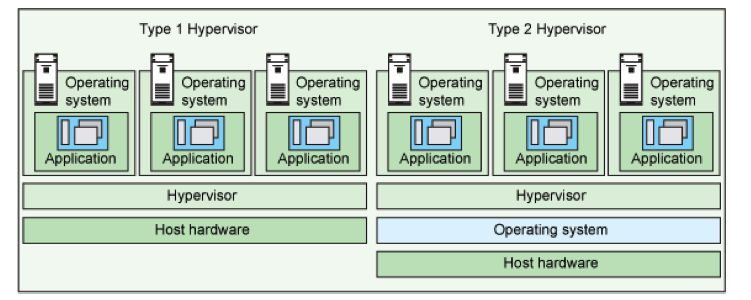
\includegraphics[scale=1]{Hypervisor}
  \caption{Hypervisor Type 1 vs. Type 2 \cite{Hypervisors}}
  \label{Hypervisor}
\end{figure}
%\vspace{-15pt}

\noindent
\textbf{Container Virtualization} 

\noindent
Container virtualization is a lightweight operating system virtualization technique that instead of trying to run an entire guest OS, it isolates the guests, but does not virtualize the hardware  \cite{container} (Figure \ref{vm vs container}). Container virtualization is considerably more lightweight than hypervisor virtualization. It has been found to be as much as 40\% less overhead using Docker based container virtualization compared to running full virtual machines on Amazon Elastic Compute Cloud (EC2) \footnote{\url{https://www.appeagle.com/ecommerce-news/ecommerce-is-on-the-rise-in-2013/}}. Each container can be treated like a regular operating system; it can be shut down, booted or rebooted. Resources such as disk space, CPU and memory associated to each container when created can be dynamically increased or decreased while the container is running and applications and users see each container as a separate host. Container virtualization allows installation of several different operating systems on top of a single kernel. Although all the operating systems use the same kernel, they have their own filesystem, processes, memory and devices \cite{container}. \\


%\vspace{-8pt}
\begin{figure}[!ht]
  \centering
     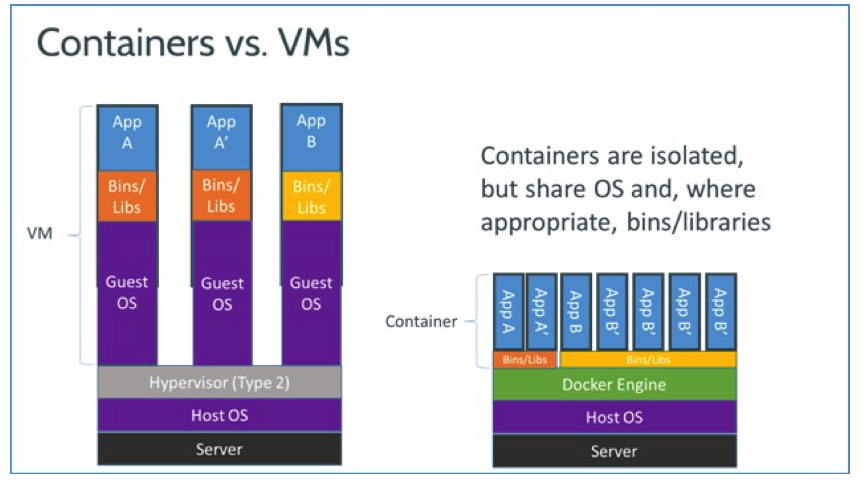
\includegraphics[scale=1]{containervsvm}
  \caption{Containers vs. Traditional Virtual Machines \textsuperscript{\ref{AAA}}}%\footnotemark %\footnotetext{\url{https://www.docker.io/the_whole_story/}} 
  \label{vm vs container}  
\end{figure}
\vspace{-18pt}

\footnotetext{ \label{AAA}\url{https://www.docker.io/the_whole_story/}} 

\noindent
\\\textbf{\textit{Linux Containers}}

\noindent
Container virtualization has been developed independently for different operating systems such as Linux OpenVZ \footnote{\url{http://openvz.org/Main_Page}}, Solaris Containers \footnote{\url{http://www.oracle.com/technetwork/server-storage/solaris/containers-169727.html}}, FreeBSD Jails \footnote{\url{http://www.freebsd.org/cgi/man.cgi?jail}}. A popular example is Linux Containers (LXC) \footnote{\label{LCX} \url{https://linuxcontainers.org/}} that allows a complete copy of the Linux OS to run in a container without the overhead of running a type-2 hypervisor. LXC uses kernel namespaces, AppArmor \footnote{\url{https://wiki.ubuntu.com/AppArmor}}, SELinux \footnote{\url{http://selinuxproject.org/page/Main_Page}}, chroots, and Control groups to provide container virtualization. 

\noindent
Kernel namespaces is used for virtualization of:

\begin{list}{-}{}
  \itemsep0em
  \item Process identifiers
  \item Network interface controllers, firewall rules and routing tables
  \item Hostname
  \item Filesystem layouts 
  \item Interprocess communication
  \end{list}

\noindent 
Control groups is used to provide:

\begin{list}{-}{}
  \itemsep0em
  \item Resource limiting to control use of resources such as memory
  \item Prioritization to control the share of the CPU being used
  \item Accounting to measure how much resources are being used
  \end{list}

\noindent
Chroots, also know as “chroot jails”, are used to change the apparent root directory in the filesystem ensuring applications cannot view files and folders outside of the chroot.

AppArmor and SELinux are used to improve security and ensure that applications cannot break out of the LXC \cite{security}.

LXC provides user environments whose resources can be tightly controlled, without the need to virtualize the hardware resources. It also allows running many copies of application configurations on the same system \footnote{\url{https://linuxcontainers.org/}}. This has proven to be a significantly useful feature of these containers for seamless software upgrade (Section \ref{upgrade1}). Furthermore, since the LXC is sharing the kernel with the host system, its processes and filesystem are completely visible from the host; however, this means that the user is limited to the modules and drivers that the container has loaded. \\

%\textsuperscript{\ref{LCX}}

\noindent
\textbf{\textit{Docker}}

\noindent
Docker is an open source application (or framework) that extend and simplifies LXC to provide Linux Containers. Docker allows easy creation of lightweight, portable, self-sufficient containers. Docker extends LXC by providing many features that make it is easier to develop, deploy, automate and share containers \footnote{\label{dockerB} \url{https://www.docker.io/the_whole_story/}}. Docker simplifies containerization supporting techniques such as Continuous Delivery by allowing a Docker container built and tested on a developer's laptop to be run anywhere. Docker containers can run on bare metal servers, virtual machines, OpenStack \footnote{\url{https://www.openstack.org/}} clusters or on a service provider's infrastructure such as Digital Ocean \footnote{\url{https://www.digitalocean.com/}}. 

Advanced Multi-Layered Unification Filesystem (AuFS) is used in Docker as their filesystem. AuFS is a layered filesystem that can transparently overlay one or more existing filesystems. A Docker AuFS consists of multiple read-only layers with a single read-write layer at the top merged together to form a single filesystem representation. When a file is modified in the container, the read-only version of the file is copied into the read-write layer using a process called copy-on-write \cite{docker2}. The copy-on-write approach means that the read-write layer only contains the files that have been modified by the container. Docker supports behaviors similar to git \footnote {\url{http://git-scm.com/}} where the read-write filesystem layer can be committed and turned into a new permanent read-only layer called an image. A new container can then be created based on this image or committed filesystem layer. A container created from the image will have a union filesystem that unifies a new copy-on-write read-write filesystem layer with the images' read-only filesystem layer and the dependent image filesystem layers beneath it. A Docker image is therefore simply a diff of changes from the previous base layers, effectively keeping the size of image files to minimum. This also means that image creators have a complete audit trail of changes from one version of a container to another (Figure \ref{docker}). 

In addition,  Docker provides a scripting language for creating containers and images based on other images. The script, called a Dockerfile, defines the differences between the new image and the previous base image. Dockerfiles allow the execution of shell commands, the configuration of processes to run when the container is started and control over the public interface of the container including exposed ports and directories. 

Docker also provides a registry of containers called the Docker Index. It allows containers to be publicly shared. The index contains images created by committing a filesystem layer and images created by the Docker Index build system using a Dockerfile \cite{docker2}.
   
With Docker, a new application on a host only needs its binaries or libraries but not a new guest OS. In addition, the same application binaries can be shared between multiple running copies of the application using a shared Docker image. If modifications are made between different versions of the application only the differences need to be maintained separately \footnote{\label{dockerC} \url{https://www.docker.io/the_whole_story/}}. \\

%\vspace{-8pt}
\begin{figure}[!ht]
  \centering
     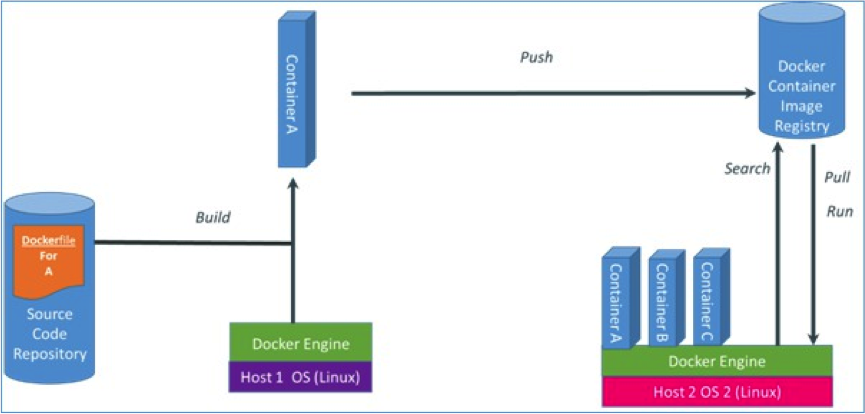
\includegraphics[scale=1]{docker}
  \caption{Basic Docker Function \textsuperscript{\ref{dockerC}}} %\footnotemark
  \label{docker}
\end{figure}
\vspace{-18pt}

%\footnotetext{\url{https://www.docker.io/the_whole_story/}} 

\subsection{CoreOS} \label{CoreOS}
CoreOS is an open source lightweight operating system based on the Linux Kernel which is designed for security, consistency and relability \footnote {\label{coreos} \url {https://coreos.com/using-coreos/}}. CoreOS does not support any package management tools such as apt \footnote{\url{https://help.ubuntu.com/12.04/serverguide/apt-get.html}} or yum \footnote {\url{http://yum.baseurl.org/}} instead it is a base OS for Docker containers. Therefore, any application can run on CoreOS, using a Docker container. CoreOS has an active/passive dual-partition scheme, similar to ChromeOS \footnote{\url{http://www.chromium.org/chromium-os}} , which is used to update the OS as a single unit instead of package by package. Initially, the system is booted into an active partition, once a new update is detected it is downloaded and installed to the passive parition. To ensure the installation does not affect the running system, it is rate limited using Linux cgroups. The system will switch to the partition with the latest update once it is rebooted \footnote {\label{coreos} \url {https://coreos.com/using-coreos/}}. CoreOS also has several tools to support simple cluster deployment including:
  \begin{list}{-}{}
  \itemsep0em
  \item \underline{etcd} - An open source distributed key value store that handles distributed locking and master election
  
  \item \underline{fleet} - A combination of systemd (a system management daemon for Linux kernal) and etcd to provide a distributed init system that supports the control of system services across a cluster. Fleet is a particularly effective method of querying and installing Docker container clusters across a CoreOS cluster.
  \end{list}

\noindent
\subsection{Messaging Systems} \label{MOM}
Messaging systems allow two or more applications to exchange information in the form of messaging. Advanced Message Queuing Protocol (AMQP) \cite{AMPQ}, Java Message Service (JMS) \cite{JMS} and Zero Message Queuing (ZeroMQ) \footnote{\label{ZeroMQ} \url{http://zeromq.org/}} are the most common messaging standards. 

\subsubsection{Broker-Based Messaging Systems} 
AMPQ and JMS are popular examples of broker-based messing systems. A message broker (also called Message Oriented Middleware) is a physical component that handles the communications between different applications. Hence, in a broker-based messaging system instead of applications directly communicating with each other, they communicate with the message broker \cite{broker}. The advantage of using this architecture is that the applications do not need to know the location of other applications. They only need to be aware of the network address of the broker. The broker then routes the messages to the correct applications based on the business requirements using the message properties, queue name or routing key \cite{AMPQ}. In addition, a broker-based messaging system is more resistant to the application failure. This is because if an application fails, messages that are already in the broker will be retained. However, broker-based messaging systems require excessive amount of network communication. Moreover, since all the messages have to be passed through the broker, the broker can turn out to be a bottleneck in the system. Therefore, the broker can be utilized to 100\% while other components of the system are under-utilized or even idle. Finally, the broker has to be managed and maintained separately to the applications sending and receiving messages. This breaks encapsulation and separation of concerns because the broker contains application specific configuration and logic. Therefore, if the application requirements change, both the broker and the application must be updated in a coordinated way. In addition, one broker often contains logic and queues for several different applications.

\subsubsection{Zero Broker Messaging Systems} 
In a broker-less messaging system each application directly talks to other applications without any middleware, hence, there are no bottlenecks associated with these systems. The application can manage and maintain its own messaging infrastructure and so encapsulation and separation of concerns are increased.

ZeroMQ is a broker-less, language agnostic, lightweight asynchronous messaging library. Asynchronous I/O model of ZeroMQ asynchronous message-processing required for scalable multi-core applications \footnote{\label{ZeroMQ} \url{http://zeromq.org/}}. 

ZeroMQ provide sockets that carry atomic messages across various transports such as Transmission Control Protocol (TCP) or User Datagram Protocol (UDP) and communication styles such as point-to-point or multicast. Unlike conventional sockets that only allow strict one-to-one, many-to-one, or in some cases one-to-many relationships, ZeroMQ sockets can be connected to multiple endpoints while simultaneously accepting incoming connections from multiple endpoints (many-to-many connection). ZeroMQ sockets support connection patterns such as request-reply (sending requests from a client to a web service or cluster of web services and receiving reply from each request sent), publish-subscribe (one-to-many distribution of data from a single publisher to multiple subscribers in a fan out manner), pipeline (distributing data to nodes arranged in a pipeline) and exclusive pair (connect one peer to exactly one other peer for inter-thread communications) patterns that is summarized in \url{http://api.zeromq.org/2-1:zmq-socket}.      

More recently, a ZeroMQ alternative, called nanomsg, has been proposed by the same team who developed ZeroMQ \footnote{\label{nanomsg} \url{http://nanomsg.org/}}. Similar to ZeroMQ, nanomsg is aimed to make the networking layer fast, scalable, and easy to use; however, it has been reported to be more lightweight than ZerMQ. In addition, in ZeroMQ each individual object is managed exclusively by a single thread. This strategy can cause issues such as inability to implement request resending in REQ/REP protocol and PUB/SUB subscriptions not being applied while application is doing other work. However, in nanomsg the objects are not tightly bound to particular threads as a result the aforementioned issues do not exist. 


\subsection{Hypertext Transfer Protocol} \label{HTTP}
The Hypertext Transfer Protocol (HTTP) is a generic, stateless application-level protocol for distributed hypermedia information systems. HTTP is the foundation protocol of the World Wide Web and it is widely used between a web browser and a web server. A feature of HTTP is the typing and negotiation of data representation, allowing systems to be built independently of the data being transferred.  To provide reliability HTTP uses TCP. Since HTTP is stateless, a new TCP connection is created between client and server for each transaction and the TCP connection terminates immediately after the transaction is completed. HTTP functions as a request-response protocol in a client-server interaction. 

\subsection{HTTP Requests} \label{Requests}
The HTTP request sent to the server by client has the following format:\\

\begin{lstlisting}[language=json,firstnumber=1]
<Request> ::=	<Request-Line>
		<general-headers>
		|<request-headers>
		| <entity-headers> CRLF
		CRLF 
		<opt-message-body>
		
\end{lstlisting} 
\noindent\\
The Request-Line consists of a method token, Request-URI and the protocol version. Method token defines HTTP functions such as GET, POST, PUT, DELETE that is performed on the resources identified by Request-URI. General headers provide general control information and they can be included in both requests and responses. Transfer-Encoding is an example of general headers which defines what (if any) type of transformation has been applied to the message body for its safe transfer between the sender and the recipient. For example if Transfer-Encoding is defined as "chunked", the data will be sent to the recipient in a series of "chunks". The request-header fields allow the client to pass additional information about the request, and about the client itself, to the server. Entity-headers define optional and required metainformation about the request body and if the request has no body, provide information about the resource identified by the request. For example, Content-Length header is one of the entity-header fields indicating the size of the request body. CRLF refers to a carriage return ('\textbackslash r') followed by a line feed ('\textbackslash n'). CRLF is used to define the end of request line and headers and start of the request body.


\subsection{HTTP Responses}
Server send HTTP responses to the client after receiving and interpreting requests using the following format: \\

\begin{lstlisting}[language=json,firstnumber=1]
<Response> ::=	<Status-Line>
		<general-headers>
		|<response-headers>
		|<entity-headers> CRLF
		CRLF 
		<opt-message-body>
\end{lstlisting} 
\noindent\\
The Status-Line consists of the HTTP version followed by a numeric status code and its associated textual phrase. Status code indicates the action taken on the corresponding request such as 'Successful' (The request was successfully received, understood, and accepted), 'Client Error' (The request contains a syntax error or the request cannot be fulfilled) and 'Server Error' (The server failed to fulfill an apparently valid request). Similar to requests, HTTP responses also have several type of headers which provides general or specific information about he response (Section \ref{Requests}). Additionally, CRLF is also used to define the end of response headers and start of the optional response body.   

 

\clearpage
\section{Design} \label{Design}
To manage the ever-increasing size of E-commerce and web related services large-scale clusters are deployed to virtualized operating systems running on hypervisors. However, hypervisors have a significant overhead when all that is required is a simple way to run clustered instances of applications. Container virtualization is considerably more lightweight than hypervisor virtualization. It has been found to be as much as 40\% less overhead using Docker based container virtualization compared to running full virtual machines on Amazon EC2 \footnote{\url{https://www.appeagle.com/ecommerce-news/ecommerce-is-on-the-rise-in-2013/}}.

In addition to the use of virtualization, continuous delivery and automated deployments are critical to reduce the cost of maintaining large clusters of software that require regular updates and feature releases. Although many companies use automated deployment tools, continuous delivery all the way into production is extremely rare due to the significant risk imposed by applying automated updates directly into production.

\subsection{Proposed Dynamic Software Update System}\label{modes} 
This project proposes a simple lightweight system to support reliable dynamic software updates suitable for continuous delivery into production. In the proposed system the updated version will run concurrently with previous stable versions. The updated system will be monitored automatically and if the system behaves incorrectly, all requests will be seamlessly routed to the previous stable version with no downtime.

Four mechanisms will be supported to enable different reliable update strategies depending on the specific software requirements.

\underline{Rapid Update} -  In this mechanism the updated version of software will immediately process all requests. The non-updated version will however remain running and will be immediately available to process requests if the updated system does not behave correctly. This mechanism is useful when an update must be applied urgently, such as a critical security patch required to stop an in-progress security breach.

\underline{New Session Update} - This update mechanism will only switch new sessions to the updated version. A new session will be identified by no requests being received from a client within a configured time period. As with Rapid Update, the non-updated version will however remain running and will be immediately available to process requests if the updated system does not behave correctly. This approach is useful when a low risk update is being made that provides features, which are important to make available to users as rapidly as possible. For example, a low risk update that is providing a new profit making service.

\underline{Long Term Update} - This mechanism will switch new sessions gradually to the updated version over multiple days or weeks. This approach is particularly useful for risky or complex updates that have a high potential to introduce system instability. This technique is also less risky since the new software version will incrementally receive a greater percentage of requests.

\underline{Multi-Version Update} - In this mechanism the updated and non-updated versions will run concurrently and  process identical requests for new sessions.  In this strategy, both the old and the new versions will handle all requests and the characteristics of each response will be compared to ensure the update is behaving correctly.

In all four mechanisms the behavior of the updated software will be automatically monitored to confirm the application is behaving correctly. The response size and delay will be compared with typical values for the non-updated version to verify the updated application behavior. Figure \ref{proposed_solution} demonstrates the component interactions within the proposed dynamic software update system.  The focus for the proposed solution will be on HTTP requests and responses.  This focus allows the use of HTTP headers to identify user sessions.  In addition, it allows efficient comparison between large responses without the need to buffer the entire response body.\\\\

%\vspace{-8pt}
\begin{figure}[!ht]
  \centering
     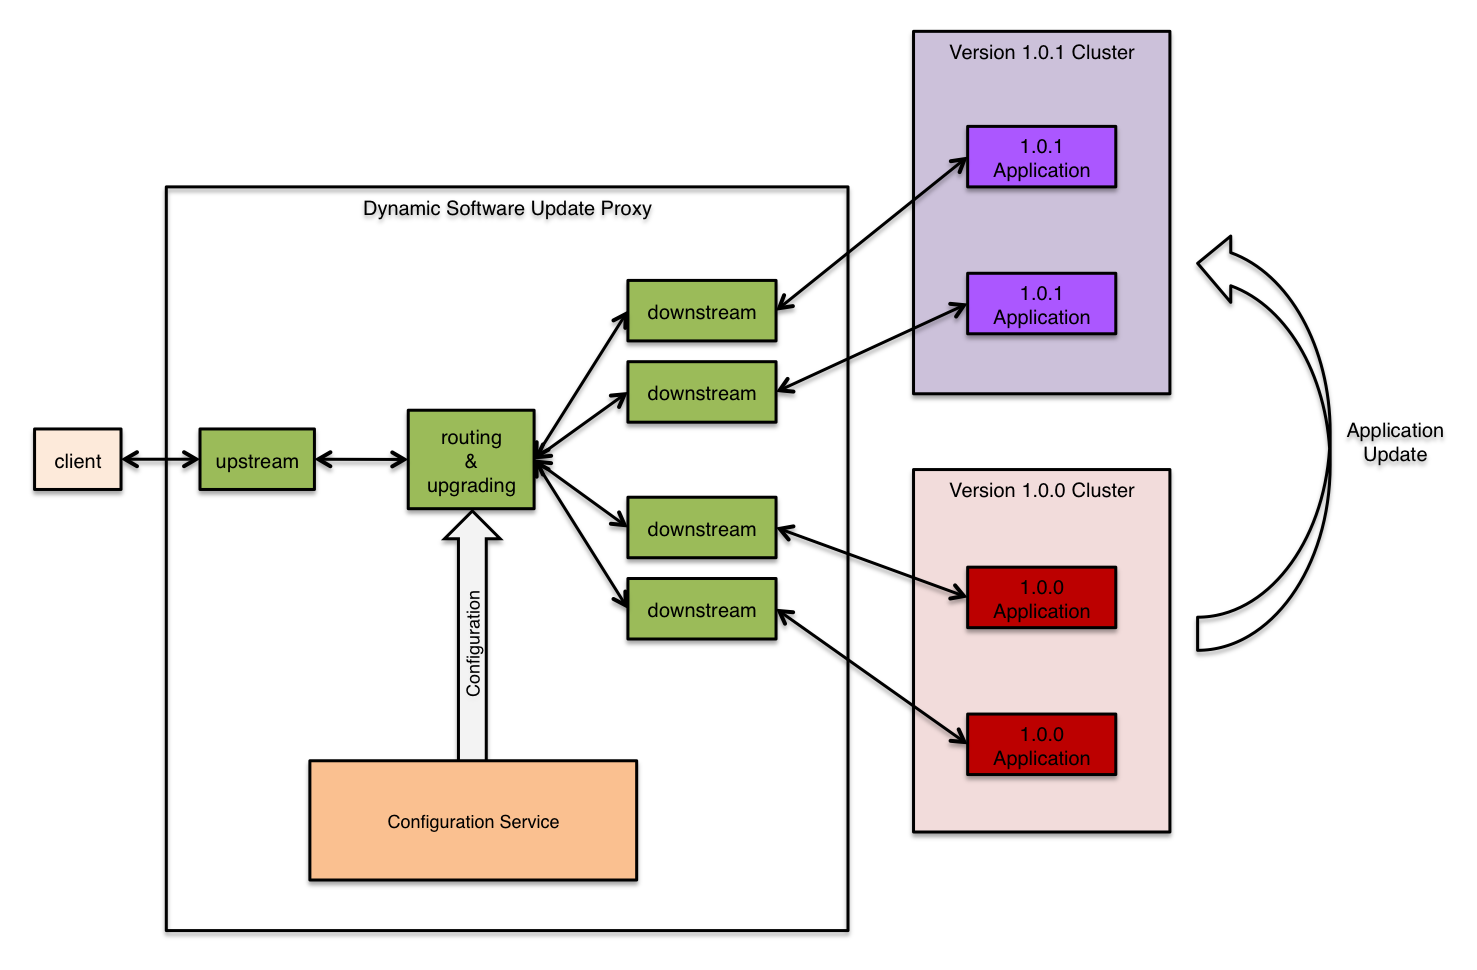
\includegraphics[scale=0.62]{proposed_solution}
  \caption{Component interactions within the proposed  dynamic software update system}
  \label{proposed_solution}
\end{figure}
%\vspace{-18pt}


\subsection{Proposed Technology Stack} 
The following technology stack has been chosen for the dynamic software update system:

\begin{list}{-}{}
  \itemsep0em
  \item Go \footnote{\url{http://golang.org/}} programming language for building proxy \textit{i.e.} the content switching load balancer. Go is chosen because of its simplicity, efficiency, scalability, highly concurrency and garbage collection. Other fast programming languages such as C\textsuperscript{++} and Java was considered to use. However, C\textsuperscript{++} was not chosen since it does not have garbage collection and requires manual memory management. Java was not chosen since it is more heavyweight in comparison to Go and it does not give the programmer control over the memory management.  
    
  \item Docker as a container virtualization mechanism that runs containers for both the target application that is to be updated and the content switching load balancer
  
  \item ZeroMQ or nanomsg as message frameworks that support highly efficient load balancing and routing of messages without the need for any middleware  

    \end{list}

\clearpage
\section{Implementation} \label{Implementation}
To produce an efficient and reliable dynamic software update system several versions of a load balancing proxy was implemented using Go programming language as described in this section. 

\subsection{Message Based Proxy Using ZeroMQ}
The first proxy developed to support dynamic software update was a HTTP reverse proxy based on ZeroMQ messaging system. A custom Dockerfile was written that creates a Docker container running an example web service using Netty \footnote{\url{http://netty.io/}}. The ZeroMQ load balancing HTTP reverse proxy uses different types of ZeroMQ sockets such as STREAM, REQ, REP and it is arranged as shown in Figure \ref{prototype}. Each box is a separate thread, a separate process or a Docker container and performs the following responsibilities:
 
\begin{list}{-}{}
  \itemsep0em
  \item \textbf{upstream} uses STREAM socket for receiving HTTP requests and replying with the HTTP response. Upstream also consists of REQ socket that forwards the requests to the router. 
  
  \item \textbf{router} is responsible for distributing requests across four downstream threads using ROUTER and DEALER sockets. ROUTER socket adds the identity of the sender and receiver to responses and requests respectively. DEALER socket distributes the requests across downstream threads in a round-robin order.
 
  \item \textbf{downstream} is responsible for receiving the requests from the router using REP sockets and sending HTTP requests to the two Docker containers containing the Netty web services and receiving the responses using STREAM socket.
\end{list}

%\vspace{-8pt}
\begin{figure}[!ht]
  \centering
     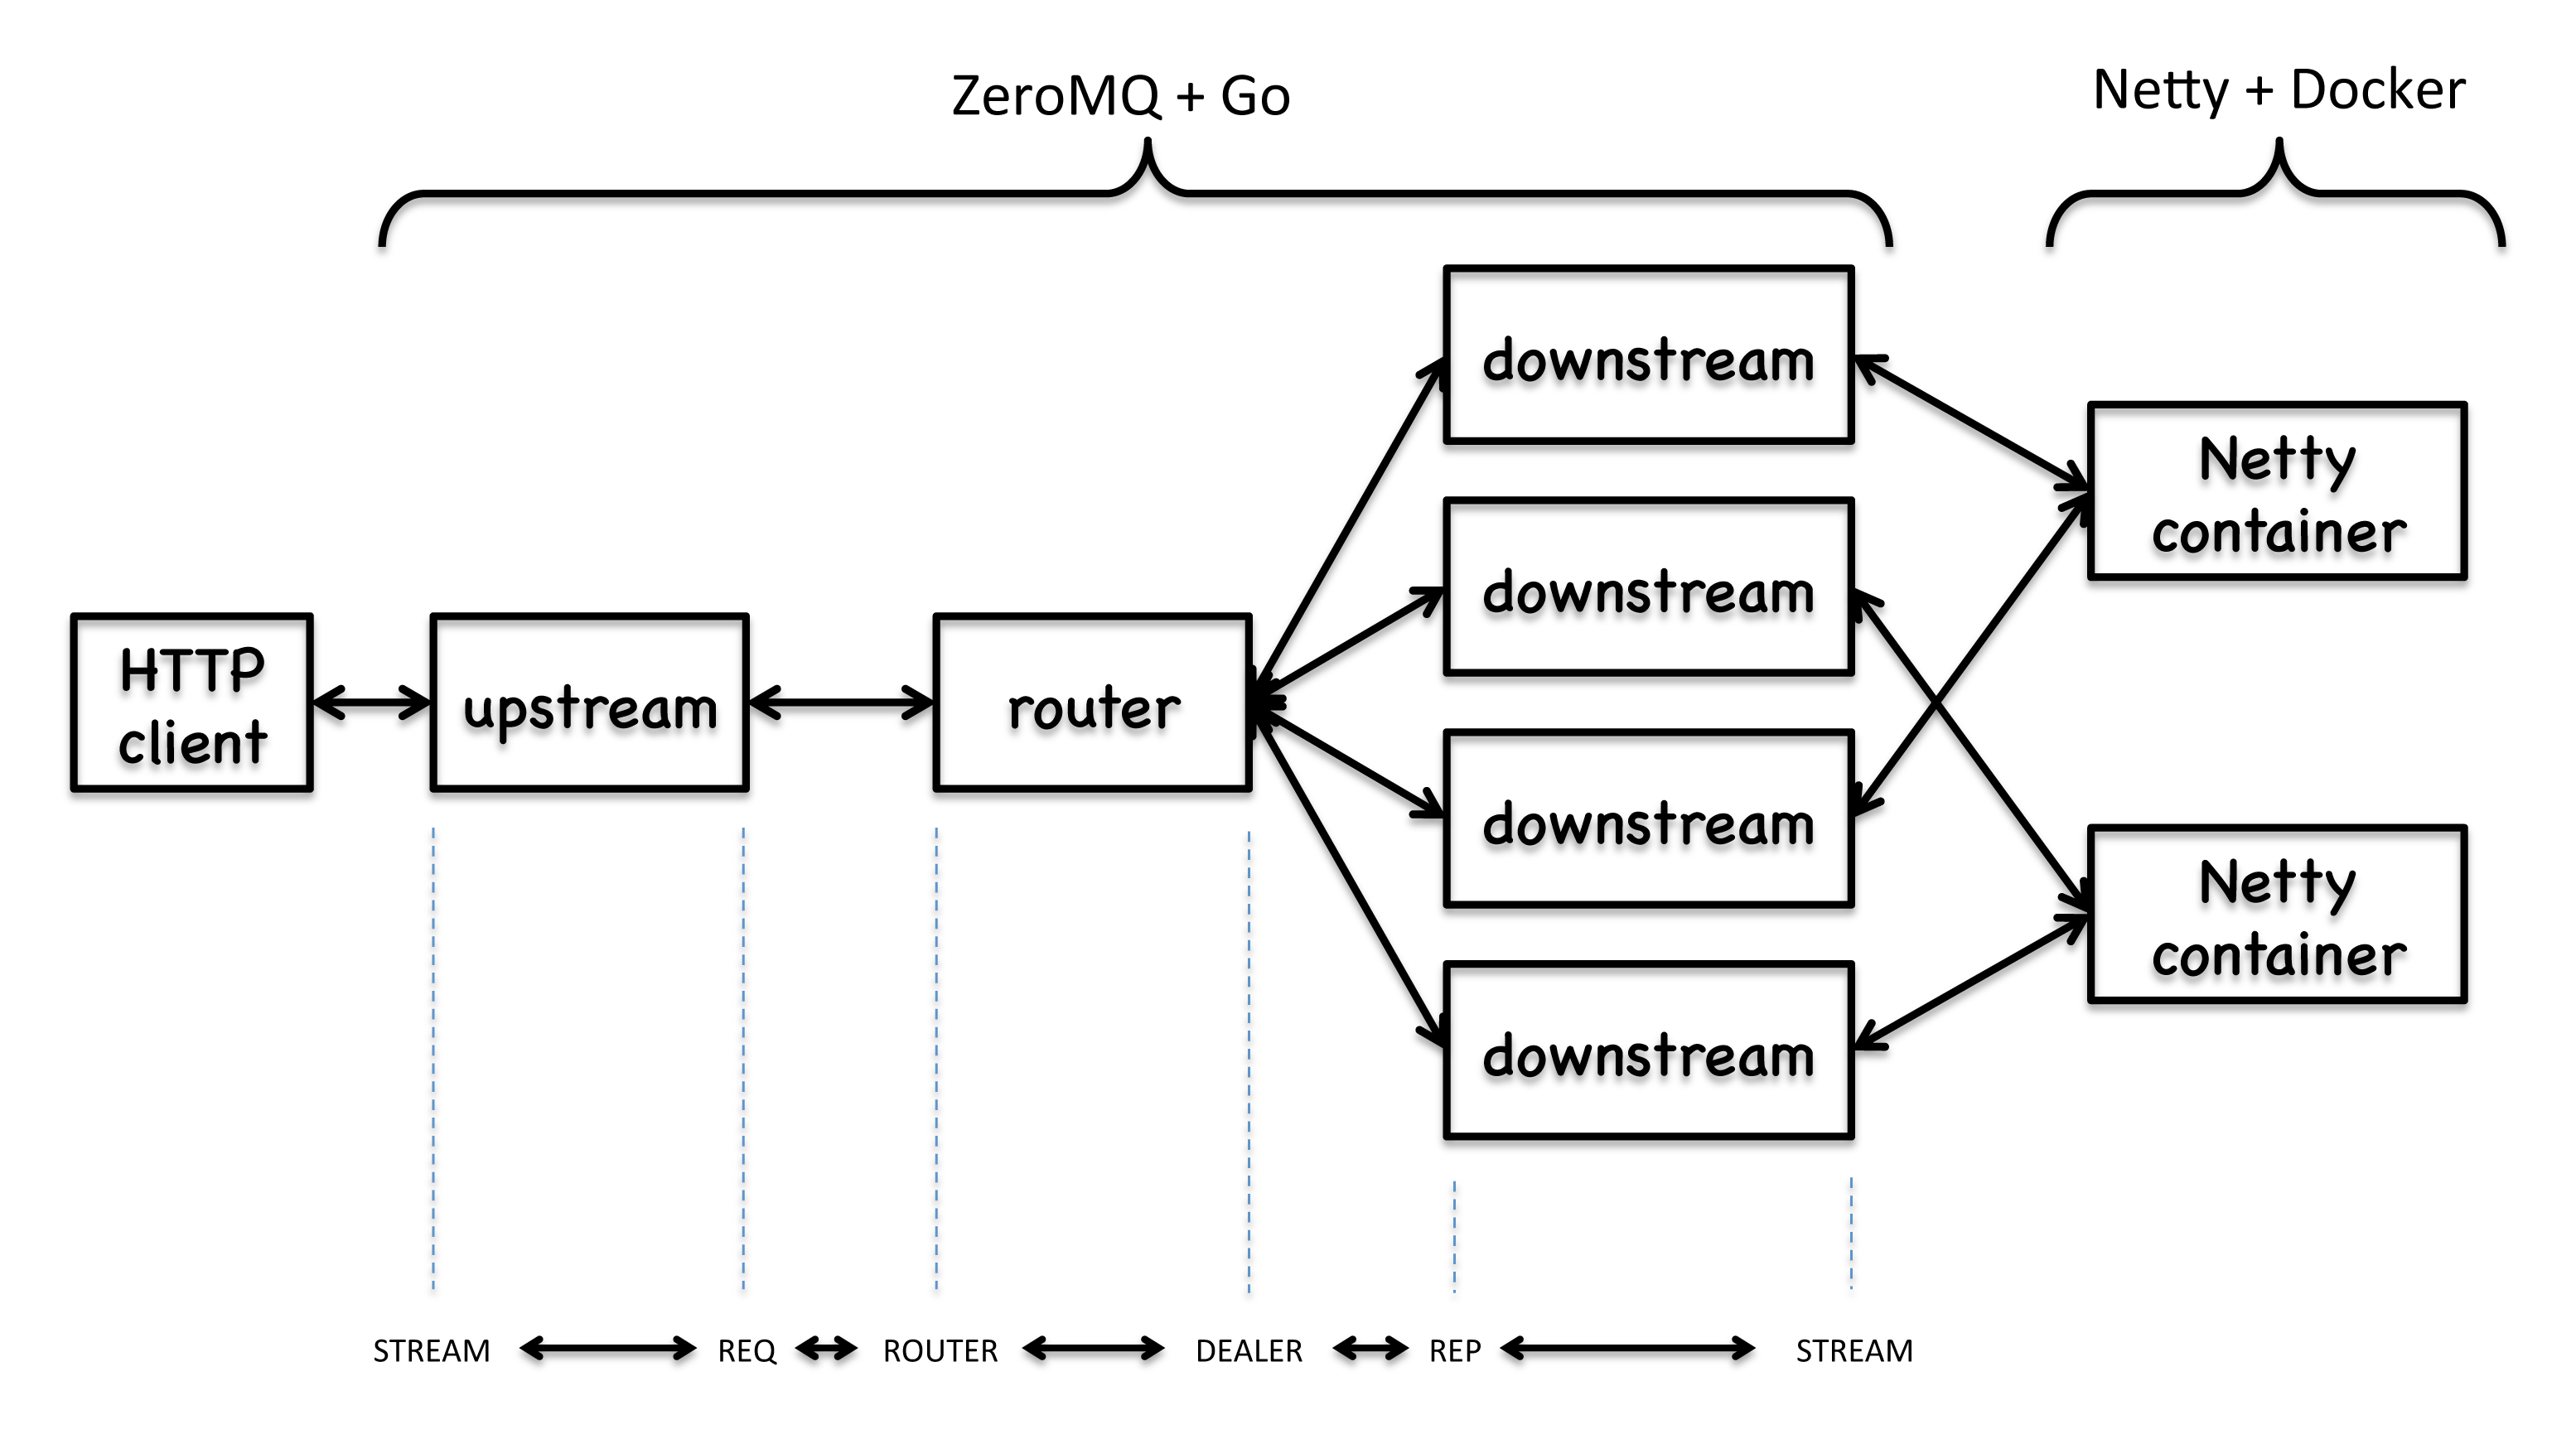
\includegraphics[scale=0.62]{prototype}
  \caption{ZeroMQ, Go and Docker Prototype}
  \label{prototype}
\end{figure}

\subsubsection{Performance Evaluation}
Detailed analysis of the reverse HTTP proxy showed that when the HTTP requests are chunked (Section \ref{Requests}), ZeroMQ STREAM socket treats each chunk as a separate message and the DEALER socket distributes each chunk of the same request to different recipients. Therefore, it was concluded that ZeroMQ messaging library is not suitable and reliable for load balancing chnuked HTTP requests and content switching load balancing can be achieved using raw Go sockets. Furthermore, HTTP provides adequate messaging support such as content encoding and caching and wrapping HTTP messages in another message layer adds unnecessary complexity and overhead. Therefore, other messaging systems such as nanomsg were not explored for developing a content switching load balancer. 

In conclusion, the ZeroMQ HTTP reverse proxy was not advanced further to support dynamic software update and an alternative one with no messaging system was sought to be developed. 

\subsection{Socket Based Proxies}
As it was explained in the previous section, a messaging system-based proxy was not the correct choice to create a reliable and efficient dynamic software update system. This section describes different approaches used to develop load balancing HTTP proxies using raw Go sockets with no messaging systems.   

\subsubsection{Socket Based Proxy With Content Counting}\label{Content-Counting}
The first version of the socket based proxy was designed as demonstrated in figure xxx. The proxy consists of a listener that listens in an  \textit{Accept} loop for new TCP connections (Figure xxx). In the case of a new connection, the listener creates a dedicated TCP connection between the client and the server. The new connection receives HTTP requests in a  \textit{Read} loop and distributes them across a cluster of HTTP services (Figure xx).  

\noindent\\
\textbf{Content Counting}\\
The content counting proxy uses HTTP format to detect the end of requests and responses \ref{HTTP}. Detecting the end of requests/responses is essential in order to reliably close Go sockets such as read and write and terminating TCP connections. 

For HTTP requests, the method token in the Request-Line is used to detect what type of HTTP function is expected (Section \ref{Requests}). If the method is defined as GET, no message body in the request is expected and the  \textit{Read} loop ends after the first read. However, for other HTTP functions such as POST or PUT and for HTTP responses, headers such as Transfer-Encoding and Content-Length were used (Section \ref{HTTP}). When the size of message body is defined by Content-Length header, proxy searches  in requests/responses for the first CRLF, which defines the end of headers and start of the message body (Section \ref{HTTP}), and it counts the length of read data after the first CRLF. When the length of read data is the same as the size defined in Content-Length header, the \textit{Read} loop terminates. However, when the Content-Length header is not set and the Transfer-Encoding header is defined as "chunked", HTTP messages are sent to the recipient in a series of chunks. At the start of each new chunk, the chunk size is defined as a hexadecimal number followed by '\textbackslash r\textbackslash n' as a line separator, therefore, the format for the last chunk is always defined as '0 \textbackslash r\textbackslash n \textbackslash r\textbackslash n'. To detect the end of HTTP messages with chunked Transfer-Encoding header, the content counting proxy screens each chunk and when the last chunk, \textit{i.e.} '0 \textbackslash r\textbackslash n \textbackslash r\textbackslash n', is detected, the  \textit{Read} loop ends. 


\noindent\\
\textbf{Performance Evaluation}\\
To evaluate the performance of the aforementioned proxy, two HTTP benchmarking tools called \textit{wrk} \footnote{\label{wrk} \url{https://github.com/wg/wrk}} and \textit{ApacheBench} (\textit{ab}) \footnote{\label{ab} \url{http://httpd.apache.org/docs/2.2/programs/ab.html}}  were used. \textit{wrk} is capable of generating significant load when it runs on a single multi-core CPU by combining a multi-threaded design and scalable event notification systems such as epoll \footnote{\label{epoll} \url{http://man7.org/linux/man-pages/man7/epoll.7.html}} and kqueue \footnote{\label{wrk} \url{http://www.freebsd.org/cgi/man.cgi?query=kqueue&sektion=2}}. \textit{ab} is a single-threaded tool used to measure the performance of HTTP web servers by generating stressing conditions.



HTTP Requests were fired to an example Go web service either directly or via the implemented content counting proxy. The processed time for each request was calculated using both \textit{wrk} and \textit{ab}. The following terminal outputs are an example of results obtained by \textit{wrk} when the benchmark was run for 2 minutes, using 400 threads and keeping 400 HTTP connections open.  \\  

\noindent
\underline{Direct HTTP Requests To Go Server}
\begin{lstlisting}[language=json,firstnumber=1]
$ ./wrk -t400 -c400 -d120 --latency http://127.0.0.1:1024
Running 2m test @ http://127.0.0.1:1024
  400 threads and 400 connections
  Thread Stats   Avg      Stdev     Max   +/- Stdev
    Latency    56.33ms    5.34ms 113.13ms   97.48%
    Req/Sec    17.26      2.09    28.00     94.61%
  Latency Distribution
     50%   55.85ms
     75%   56.36ms
     90%   56.89ms
     99%   97.85ms
  854993 requests in 2.00m, 126.38MB read
Requests/sec:   7123.93
Transfer/sec:      1.05MB
\end{lstlisting}

\noindent\\
\underline{HTTP Requests To Go Server Via Content Counting Proxy} 
\begin{lstlisting}[language=json,firstnumber=1]
$ ./wrk -t400 -c400 -d120 --latency http://127.0.0.1:1234
Running 2m test @ http://127.0.0.1:1234
  400 threads and 400 connections
  Thread Stats   Avg      Stdev     Max   +/- Stdev
    Latency   381.51ms  131.93ms 482.79ms   83.01%
    Req/Sec     0.48      2.34    26.00     95.10%
  Latency Distribution
     50%  472.32ms
     75%  480.15ms
     90%  481.42ms
     99%  482.69ms
  25835 requests in 2.00m, 3.82MB read
  Socket errors: connect 0, read 27144, write 681, timeout 21088
Requests/sec:    215.24
Transfer/sec:     32.58KB
\end{lstlisting}


\noindent \\
The above results show that significant socket errors such as read and write errors occur when the requests are sent to the Go server via proxy. The socket errors consequently reduce the number of requests processed by the server (\textit{e.g.} from 7123.93/second to  215.24/second), the amount of data transferred (\textit{e.g.} from 1.05MB/second to 32.58KB/second) and finally increases the time taken for each request to be processed (average time increased from 56.33ms to 381.51ms). The results obtained from \textit{wrk} were consistent and similar results were obtained when \textit{ab} was used for evaluations. Detailed analysis of the proxy showed that the content counting proxy is not persistantly detecting the end of messages, therefore, the read and write sockets do not close appropriately which results in socket errors. 

In conclusion, the significant overhead and socket errors associated with the implemented proxy lead us think that a proxy with content counting is not suitable for supporting reliable and efficient dynamic software updates. Therefore, another version of the socket based proxy was developed as described in the next section.

\subsubsection{Socket Based Staged Proxy With End Of File Signal}\label{staged}
The final version of the socket based proxy was implemented using a Stage Based Design (SBD) as demonstrated in figure \ref{proxy}. The SBD  approach was used to improve the code design, simplicity and to support good test coverage. Additionally, the SBD also promoted encapsulation, separation-of-concerns and allowed inversion-of-control and dependency-injection which resulted in the following benefits:

\begin{list}{-}{}
  \itemsep0em
  \item\textbf{Encapsulation And Separation Of Concerns} - resulted in separating logic for each functional area into a single component. This creates a simple and isolated code that focuses on one topic, making it clear and easier to understand. Additionally, encapsulation and separation of concerns simplified testing by allowing each test to be focused on one specific area. For example, multiple tests could be done on reading from a socket and dealing with different errors and situation that can occur to insure a reliable reading process unlike the unreliable  \textit{Read} loop described in section \ref{Content-Counting}. 

  \item\textbf{Inversion-Of-Control And Dependency Injection} - allowed incremental development of the proxy where new components were plugged-in and configured one by one while existing components all worked together. For the HTTP load balancing proxy shown in figure \ref{proxy} the  \textit{Read} and  \textit{write} stages were first developed. That was followed by development of the  \textit{Complete} and  \textit{Route} stages respectively and then the rest of proxy was implemented. This approach also simplified testing of the proxy for the following reasons:
\begin{list}{-}{}
  \itemsep0em
  \item allowing the code-under-test to be isolated by mocking all dependencies 
  
  \item allowing the mocking of different error situations that would be impossible to test without mocking dependencies
  
\end{list}

\end{list}

\noindent
To prevent socket errors occured in the content counting proxy \ref{Content-Counting}, the staged HTTP load balancing proxy uses the End-Of-File (EOF) signal to detect the end of messages instead of content counting. Different component and stages of the proxy is shown in figure \ref{proxy} and their functionality is explained below.\\

\begin{figure}[!ht]
  \centering
     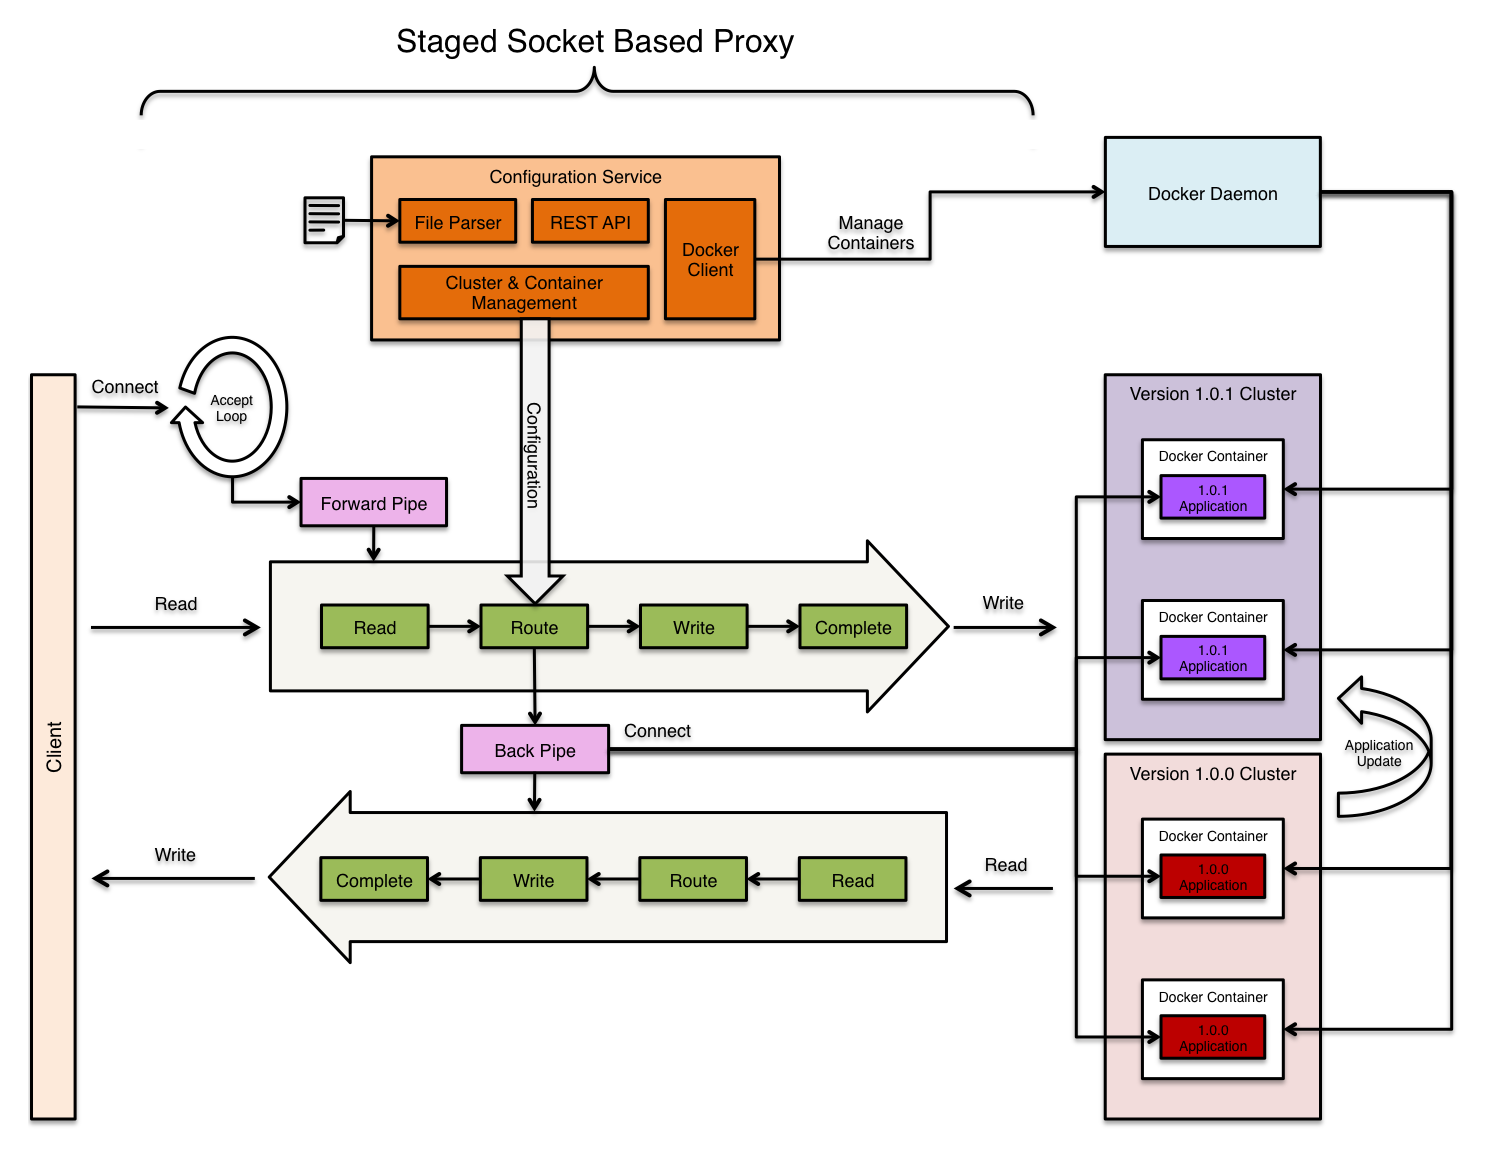
\includegraphics[scale=0.60]{proxy}
  \caption{Socket Based Staged Proxy Design Supporting Dynamic Software Update}
  \label{proxy}
\end{figure}
% \vspace{-18pt}

\noindent
\textbf{Accept Loop} \\
 \textit{Accept} loop accepts incoming HTTP connections on a listener and creates a  \textit{Forward pipe} for each request.\\  

\noindent
\textbf{Forward Pipe} \\
\textit{Forward pipe} constructs the \textit{ChunkContext Struct} for the received request and creates \textit{Read}, \textit{Route}, \textit{Write} and \textit{Complete} stages of the proxy for forwarding the request to the appropriate server in the cluster. The \textit{ChunkContext Struct} is used to encapsulate the information for managing the transferring chunks of data between the client and servers of the proxy. The \textit{ChunkContext} contains information such as network addresses of the client and the server and the data transfer direction, as follows: \\ 

\begin{lstlisting}[language=json,firstnumber=1]
type ChunkContext struct {
	Data                   []byte
	To                     tcp.TCPConnection
	From                   tcp.TCPConnection
	Err                    error
	TotalReadSize          int64
	TotalWriteSize         int64
	PipeComplete           chan int64
	FirstChunk             bool
	RoutingContext         *RoutingContext
	Direction              Direction
}
\end{lstlisting} 

\noindent\\
\textbf{Read Stage} \\
\textit{Read} stage is responsible for reading input in a loop from the HTTP connection. The \textit{Read} stage in \textit{Forward pipe} reads requests from the client, while the one in \textit{Back pipe} reads responses from the server. The \textit{Read} loop terminates when an error is encountered while reading from a socket. In the staged proxy (Figure \ref{proxy}) when an EOF condition (\textit{i.e.} when no more input is available)  occurs, \textit{Read} treats this condition as an error and it stops reading from the connection. This approach allows a graceful and efficient way of detecting the end of input. It also prevents the need for parsing requests/responses and the content counting process mentioned in section \ref{Content-Counting}, which is very inefficient and unreliable.\\

\noindent
\textbf{Route Stage} \\
\textit{Route} stage has different functionality in the \textit{Forward Pipe}, \textit{i.e.} processing requests and \textit{Back pipe}, \textit{i.e.} processing responses. \\   

\noindent
\underline{Routing in \textit{Forward Pipe}} - When a new request arrives in the \textit{Route} stage, the \textit{Route} checks the upgrade transition mode of the most updated cluster and forwards the request chunks to the correct instance of the cluster accordingly. Currently the proxy supports four different upgrade transition modes; INSTANT, SESSION, GRADUAL and CONCURRENT (Section \ref{modes}). The \textit{Route} stage distributes the requests using the modes according to the rules summarized below: 

\begin{list}{-}{}
  \itemsep0em
  \item{\textbf{INSTANT}} - If the upgrade transition mode in the most updated version of the cluster is defined as INSTANT, \textit{Route} stage forwards the requests to the latest cluster. If no upgrade transition is defined in the cluster configuration, INSTANT mode will be the default mode (Section \ref{PUT}).\\
  
  \item{\textbf{SESSION}} -  When upgrade transition mode of a cluster is defined as SESSION, the proxy will generate a  session cookie with a configured expiry time for each request forwarded to that cluster. The session cookie will be added as a header to the HTTP response using  Set-Cookie. If the request arrived in \textit{Route} stage has an assigned cookie and it is not timed out, \textit{Route} stage forwards the request to the cluster associated with the cookie, otherwise requests will be forwarded according to the upgrade transition mode of the cluster with highest version number. If the cluster configuration has an upgrade transition but the mode is not defined, SESSION mode will be assigned to that cluster. \\
  
   \item{\textbf{GRADUAL}} - When a client connects to a cluster with GRADUAL transition mode, a transition cookie will be added to responses associated to that client. The transition cookie refers to a percentage determining when the client should switch to the new version of the system. As an example, if the transition percentage is 15\%, this means that the \textit{Route} stag forwards the first 15\% of the requests to the old version before forwarding the requests to the new version.\\
   
   \item{\textbf{CONCURRENT}} - When the upgrade transition mode is set to CONCURRENT, the \textit{Route} stage forwards requests concurrently to the two most updated cluster versions.        
\end{list}
\noindent
If the user decide to delete the updated version of the cluster or an error occurs while routing the requests to a cluster, the request will be forwarded to the older version of the cluster. If routing to all versions failed, the process stops and returns an appropriate error to the client. If the request is successfully routed, a \textit{Back pipe} will be created by \textit{Route} stage for processing responses.   

\noindent\\
\underline{Routing in \textit{Back pipe}} - The \textit{Route} stage processes responses differently according to the configuration of the cluster which the response is originated from. If the upgrade transition mode in the cluster is defined as INSTANT, the response will be sent to the client with no further modifications. If the mode is set to SESSION or GRADUAL, \textit{Route} stage sets the session cookie or the transition cookie to the response respectively before forwarding it to the client. Finally, if the mode is defined as CONCURRENT, the response from each cluster version will be parsed and HTTP headers such as status code, Transfer-Encoding, Content-Length and the response delays are compared. If the characteristics  of the response from the new cluster is identical to the old one, only the response from the new version will be send to the client. Otherwise the response from the new version will be dropped and the old version's response will be used.\\

\noindent
\textbf{Write Stage} \\
\textit{Write} stage writes received requests/responses to an underlying data stream. The writing process stops if any errors such as \textit{ErrShortWrite} encountered while writing to a socket. The \textit{Write} stage in \textit{Forward pipe} writes data to the server, while the \textit{Write} stage in \textit{Back pipe} writes data to the client.   \\

\noindent
\textbf{Complete Stage}\\ 
\textit{Complete} stage is responsible for shutting down the writing and reading sides of the TCP connection when the \textit{Read} and \textit{Write} stages terminate. This is done to insure that a TCP connection is reliably closed when the client/server communication is ended. This proved to be essential for generating a fast and reliable dynamic software update system.\\ 

\noindent
\textbf{Back Pipe}\\
\textit{Back pipe} is responsible for receiving requests from the server and forwarding it to the client. Similar to \textit{Forward pipe}, \textit{Back pipe} constructs the \textit{ChunkContext Struct} for the received response and creates \textit{Read}, \textit{Route}, \textit{Write} and \textit{Complete} stages for forwarding the response to the client.\\\\

xxxxxxxx\\\\
HAVE A DIAGRAM ABOUT COMPARING ALL THREE PROXIES AND SAY THEREFORE THE LAST VERSION WAS USED FOR FURTHERER ADVANCEMENT\\\\

XXXXXXXXX\\



\subsection{Proxy Installation}
The proxy can be installed in two simple steps as follows:
\begin{list}{-}{}
  \itemsep0em
  \item git clone \url {https://github.com/samirabloom/dynamic-software-update} 
  \item make
\end{list}

\noindent
The above steps install the proxy to the PATH by adding it to the \textit{/usr/local/bin} directory. However, this will only work if the PATH environment variable has \textit{/usr/local/bin} in its list of directories. 

\subsection{Command Line Interface}
The proxy runs from the command line with the following options:\\

\begin{lstlisting}[language=json,firstnumber=1]
Usage of proxy:
  -configFile="./config.json":  Set the location of the configuration file 
  that should contain configuration to start the proxy, 
  for example:
              {
                  "proxy": {
                      "port": 1235
                  },
                  "configService": {
                      "port": 9090
                  },
                  "cluster": {
                      "servers":[
                          {"ip": "127.0.0.1", "port": 1034},
                          {"ip": "127.0.0.1", "port": 1035}
                      ],
                      "version": 1.0
                  }
              }

  -logLevel="WARN":  Set the log level as "CRITICAL", "ERROR", "WARNING", 
  "NOTICE", "INFO" or "DEBUG"

  -h: Displays this message
\end{lstlisting} 

\noindent\\
For example the following command will run the proxy in the "INFO" log level and uses a file called \textit{config/config\_script.json} for its configuration. 

\begin{lstlisting}[language=json,firstnumber=1]
proxy -logLevel=INFO -configFile= "config/config_script.json" 
\end{lstlisting}
 
\subsection{REST API}
The proxy provides a simple REST API (Figure \ref{proxy}) to support dynamically updating the cluster configuration as follows:

\begin{list}{-}{}
  \itemsep0em
  \item\textbf{{PUT /configuration/cluster}} - adds a new cluster configuration
  
  \item\textbf{{GET /configuration/cluster/{clusterId}}} -  gets a single cluster configuration
  
   \item\textbf{{GET /configuration/cluster}} - gets a list of all cluster configurations
   
   \item\textbf{{DELETE /configuration/cluster/{clusterId}}} -  deletes a single cluster configuration
  
\end{list}
\noindent
The REST API supports the following HTTP response codes:

\begin{list}{-}{}
  \itemsep0em
  \item{202 Accepted}  -  a new cluster entity is successfully added or deleted
  
  \item{200 OK} -  cluster(s) entity is successfully returned
  
   \item{404 Not Found} - cluster id is invalid
   
    \item{400 Bad Request } - request syntax is invalid
  
\end{list}

\subsubsection{PUT /configuration/cluster}\label{PUT}
The PUT request to \textit{/configuration/cluster}  is used to add a new cluster to the proxy. The format of the request body is as follows:\\

\begin{lstlisting}[language=json,firstnumber=1]
{
    "cluster": {
        "servers": [
            {
                "ip": "", 
                "port": 0
            }
        ], 
        "version": 0, 
        "upgradeTransition": {
            "mode": ""
            "sessionTimeout": 0  
            "percentageTransitionPerRequest": 0
            "percentageTransitionPerRequest": 0  
        }
    }
}
\end{lstlisting}

\noindent\\
The JSON fields are used for the following reasons:

\begin{list}{-}{}
  \itemsep0em
  \item\textbf{{cluster.servers}} - specifies the list of servers in the cluster.
  
  \item\textbf{{cluster.servers[i].ip}} - specifies the IP address or hostname of a server in the cluster.
  
  \item\textbf{{cluster.servers[i].port}} - specifies the port of a server in the cluster.
  
  \item\textbf{{cluster.version}} - specifies the cluster version. 
  
  \item\textbf{{cluster.upgradeTransition}} - allows the configuration of the upgrade transition. If no \textit{upgradeTransition} is specified, the upgrade transition mode defaults to INSTANT.  
  
  \item\textbf{{cluster.upgradeTransition.mode}} - specifies the upgrade transition mode and support the following values: INSTANT, SESSION, GRADUAL and CONCURRENT.
   
  \item\textbf{{cluster.upgradeTransition.sessionTimeout}} - specifies the timeout period assigned to the SESSION transition mode.
  
  \item\textbf{{cluster.upgradeTransition.percentageTransitionPerRequest}} - specifies the transition percentage associated with each request in the GRADUAL transition mode.
\end{list}

\noindent
When the user send a PUT request and successfully adds a new cluster, the proxy responds by returning a cluster id representing the new cluster entity that has been added. Appendix \ref{Appendix  I} demonstrates detailed examples of the PUT requests and responses supported by proxy and the type of values that can be used in each field of the message body.

\subsubsection{GET - /configuration/cluster/\{clusterId\}} 
GET requests to \textit{/configuration/cluster/\{clusterId\}} gets a single cluster configuration. If no cluster id is specified and the GET request is sent to \textit{/configuration/cluster/}, a list of all the cluster configurations added to the proxy will be returned. The format of the response body for getting a cluster configuration with a specific cluster entity is shown below and detailed examples of GET requests and responses are demonstrated in Appendix \ref{Appendix  I}.\\

\begin{lstlisting}[language=json,firstnumber=1]
{
    "cluster": {
        "servers": [
            {
                "ip": "",
                "port": 0
            }
        ],
        "upgradeTransition": {
                "mode": ""
                "sessionTimeout": 0  
                "percentageTransitionPerRequest": 0  
        },
        "uuid": "",
        "version": 0
    }
}

\end{lstlisting}

\subsubsection{DELETE - /configuration/cluster/\{clusterId\}}
DELETE requests to \textit{/configuration/cluster/\{clusterId\}} deletes a single cluster configuration. No request body and response body is defined for the DELETE request. Appendix \ref{Appendix I} shows an example of a DELETE request and the response received from the proxy.

\subsection{Testing}
As explained by the previous sections, the proxy consists of many components. Therefore, several testing strategies were used to suit the needs of each component (Figure xxxxxxx).\\

XXXXXXXXXXXXXXXXXXXXXXXXXXXXXXXXXXXXXXXXXXXXXXXXXXXXXXXX\\
XXXXXXXX A FIGURE FOR TESTING XXXXXXXXXXXXXXXXXXXXXXXXXXXXX\\
XXXXXXXXXXXXXXXXXXXXXXXXXXXXXXXXXXXXXXXXXXXXXXXXXXXXXXXX\\ 

\subsubsection{Unit Testing}
These tests focus on low level checking of the functionality of each proxy component. Inversion-of-control and dependency-injection (Section \ref{staged}) allowed dependencies to be injected into each component and be mocked. The unit tests cover both positive and negative cases resulting in overall of xxxxxxx line coverage and xxxxxxx branch coverage.    

XXXXXXXXXXXXXXXXXXXXXXXXXXXXXXXXXXXXXXXXXXXXXXXXXXXXXXXX\\
XXXXXXXX MAYBE ADD A SCREEN SHOT XXXXXXXXXXXXXXXXXXXXXXXXXXXXX\\
XXXXXXXXXXXXXXXXXXXXXXXXXXXXXXXXXXXXXXXXXXXXXXXXXXXXXXXX\\ 


\subsubsection{Integration Testing}
These testes focus on the integration between different components of the REST API and the poxy. To ensure each component of the REST API integrates correctly, tests were designed to send simultaneous PUT, GET and DELETE requests to the REST server and the responses were analyzed. In addition, integration of different stages of the proxy was tested using different scenarios such as testing the behavior of when the proxy is configured for SESSION or CONCURRENT upgrade or when a cluster configuration is deleted from the proxy.

\subsubsection{System Testing}
The aim of these tests is to check that the components of the dynamic software update system including proxy and the REST API work together. System tests were written to cover complete user scenarios. The tests are executed by starting the proxy with an initial configuration. Then HTTP requests is fired at the proxy and the test checks that the proxy is distributing the requests to the cluster of servers correctly. Afterwards, the four different upgrade modes described in section \ref{modes} are applied via the REST API and the behavior of the  proxy is tested. Finally, the proxy is tested when clusters are deleted from the proxy.   

\subsection{Dockerising the proxy}
Talk about how I dockerised the proxy\\\\
why didn't use fleet system and coreOS? \\\\





\clearpage
\section{Evaluation}
The system to support dynamic software update will be evaluated as described below.

\subsection{Qualitative Analysis}
\noindent
\underline{Handling Incorrect Behavior } - To ensure that the system is able to handle updates that cause incorrect behavior multiple scenarios will be tested. This test will cover situations where a single node, multiple nodes or all nodes in the updated application cluster behave incorrectly. Incorrect behavior will be modeled by either the application crashing or by the application taking too long to respond.

\noindent
\underline{Automated Software Update} - To prove the suitability of the proposed system for continuous delivery, application updates will be performed using both a bash script \footnote{\url{http://www.tldp.org/LDP/abs/html/}} and a puppet manifest \footnote{\url{https://puppetlabs.com/}}. Puppet has been chosen since it is the most widely used automated deployment tool. In addition bash has been chosen since all automated deployment tools have the ability to run bash commands. 


\subsection{Quantitative Analysis}
\noindent
\underline{Load Test} - A load test will be used to measure the performance as the number of requests increases. This test will demonstrate the delay incurred by the content switching load balancer and the maximum number of requests that the system can handle.

\noindent
\underline{Saturation Test} - This test will be performed to measure the performance of the system when it is has been exposed to a moderate number of requests over a prolonged period of time. This test will demonstrate that the system can run for a prolonged period of time without any degradation, such as memory leaks.

\noindent
\underline{Update Speed} -Rapid Updates will be performed to measure how quickly the requests will be transferred to the updated version of the software. 

\noindent
\underline{Software Recovery} - Bugs will be introduced to the new version of the software to calculate the speed of switching to the non-updated version.


\clearpage
\section{Conclusions \& Future Plans}
xxxxxxxxx\\
xxxxxxxxx\\
xxxxxxxxx\\


\clearpage
\section{Appendices}

\subsection{Appendix I: Proxy REST API}\label{Appendix I}
The proxy provides a simple REST API to support dynamically updating the cluster configuration as follows:

\begin{list}{-}{}
  \itemsep0em
  \item \textbf{PUT /configuration/cluster} - adds a new cluster configuration  
 \item\textbf{GET /configuration/cluster/{clusterId}} - gets a single cluster configuration
 \item\textbf{GET /configuration/cluster} - gets all cluster configurations
 \item\textbf{DELETE /configuration/cluster/{clusterId}} - deletes a single cluster configuration
\end{list}

\noindent
\textbf{HTTP Response Codes}
\begin{list}{-}{}
  \itemsep0em
\item 202 Accepted - a new cluster entity is successfully added or deleted 
\item 200 OK - cluster(s) entity is successfully returned   
\item 404 Not Found - cluster id is invalid
\item 400 Bad Request - request syntax is  invalid
\end{list}

\noindent
\textbf{PUT - /configuration/cluster}\\
To add a new cluster make a PUT request to \textit{/configuration/cluster}.\\

\noindent
\textit{\textbf{Request Body}}
 
\begin{lstlisting}[language=json,firstnumber=1]
{
  "cluster": {
    "servers": [
      {
        "ip": "",
        "port": 0
      }
    ],
    "version": 0,
    "upgradeTransition": {
        "mode": ""  // allowed values are "INSTANT", "SESSION", "GRADUAL", "CONCURRENT"
        "sessionTimeout": 0  // only supported for a 'mode' value of "SESSION" 
        "percentageTransitionPerRequest": 0  // only supported for a 'mode' value of "GRADUAL"
      }
    }
}
\end{lstlisting}
\noindent \\
\textbf{cluster.servers}\\
\noindent
Type: 'Array'  Default value: '[]'\\
\noindent
This value specifies the list of servers in the cluster\\

\noindent
\textbf{cluster.servers[i].ip}\\
\noindent
Type: 'String' Default value: 'undefined'\\
\noindent
This value specifies the ip address or hostname of a server in the cluster\\

\noindent
\textbf{cluster.servers[i].port}\\
\noindent
Type: 'Number' Default value: 'undefined'\\
\noindent
This value specifies the port of a server in the cluster\\

\noindent
\textbf{cluster.version}\\
\noindent
Type: 'Number' Default value: '0'\\
\noindent
This value specifies the cluster version. If no version is specified, the version defaults to '0'. \\

\noindent
\textbf{cluster.upgradeTransition}\\
\noindent
Type: 'Object' Default value: ''INSTANT'\\
\noindent
This value allows the configuration of the upgrade transition. If no 'upgradeTransition' is specified, the upgrade transition mode defaults to 'INSTANT'.\\

\noindent
\textbf{cluster.upgradeTransition.mode}\\
\noindent
Type: 'String' Default value: 'SESSION'\\
\noindent
This value specifies the upgrade transition mode and support the following values: 'INSTANT', 'SESSION', 'GRADUAL', 'CONCURRENT'.\\

\noindent
\textbf{cluster.upgradeTransition.sessionTimeout}\\
\noindent
Type: 'Number' Default value: 'undefined'\\
\noindent
This value specifies the timeout period assigned to the 'SESSION' transition mode. \\

\noindent
\textbf{cluster.upgradeTransition.percentageTransitionPerRequest}\\
\noindent
Type: 'Number' Default value: 'undefined'\\
\noindent
This value specifies the transition percentage associated with each request in the `GRADUAL` transition mode. \\

\noindent
\textbf{Response Body}\\
\noindent
A cluster id is returned representing the new cluster entity that has been added. \\

\noindent
\textbf{Example}\\

\noindent
\textbf{Request}\\
\noindent
For example the following JSON would set up a new cluster with two 'servers' and 'SESSION' upgrade transition:

\begin{lstlisting}[language=json,firstnumber=1]

{
  "cluster": {
    "servers": [
      {
        "ip": "127.0.0.1", 
        "port": 1036
      },  
      {
        "ip": "127.0.0.1", 
        "port": 1038
      }
    ], 
    "version": 1.1, 
    "upgradeTransition": {
      "mode": "SESSION", 
      "sessionTimeout": 60
    }
  }
}
\end{lstlisting}

\noindent \\
To send this request with 'Curl' use the following syntax:\\

\begin{lstlisting}[language=json,firstnumber=1]
curl http://127.0.0.1:9090/configuration/cluster -X PUT --data '{"cluster": {"servers":[{"ip": "127.0.0.1", "port": 1036},{"ip": "127.0.0.1", "port": 1038}],"version": 1.1,"upgradeTransition": { "mode": "SESSION", "sessionTimeout": 60 }}}'
\end{lstlisting}

\noindent \\
\textbf{Response}\\

\begin{lstlisting}[language=json,firstnumber=1]
HTTP/1.1 202 Accepted
Date: Sat, 16 Aug 2014 19:54:21 GMT
Content-Length: 36
Content-Type: text/plain; charset=utf-8
 
1dcbb083-257f-11e4-bcbc-600308a8245e
\end{lstlisting}

\noindent \\
\textit{\textbf{GET - /configuration/cluster/{clusterId}}}\\

\noindent 
To get a single cluster configuration make a GET request to \textit{/configuration/cluster/{clusterId}}.\\ 

\noindent 
\textbf{Response Body}\\

\begin{lstlisting}[language=json,firstnumber=1]
{
  "cluster": {
    "servers": [
      {
        "ip": "",
        "port": 0
      }
    ],
    "upgradeTransition": {
      "mode": ""
      "sessionTimeout": 0  // only returned when 'mode' is "SESSION" 
      "percentageTransitionPerRequest": 0  // only returned when 'mode' is "GRADUAL"
    },
    "uuid": "",
    "version": 0
  }
} 
\end{lstlisting}

\noindent \\
\textbf{Example}

\noindent \\
\textbf{Request}

\noindent 
For example the following 'curl' request would get the cluster configuration with cluster id '1dcbb083-257f-11e4-bcbc-600308a8245e':\\

\begin{lstlisting}[language=json,firstnumber=1]
curl http://127.0.0.1:9090/configuration/cluster/1dcbb083-257f-11e4-bcbc-600308a8245e -X GET
\end{lstlisting}

\noindent \\
\textbf{Response}\\

\begin{lstlisting}[language=json,firstnumber=1]
{
  "cluster": {
    "servers": [
      {
        "ip": "127.0.0.1",
        "port": 1036
      },
      {
        "ip": "127.0.0.1",
        "port": 1038
      }
     ],
    "upgradeTransition": {
        "mode": "SESSION",
        "sessionTimeout": 60
    },
    "uuid": "016ca2cd-2585-11e4-ab5c-600308a8245e",
    "version": 1.1
  }
}
  
\end{lstlisting}

\noindent \\
For example the response when using curl is as follows:

\begin{lstlisting}[language=json,firstnumber=1]
HTTP/1.1 200 OK
Date: Sat, 16 Aug 2014 20:37:42 GMT
Content-Length: 206
Content-Type: text/plain; charset=utf-8

{"cluster":{"servers":[{"ip":"127.0.0.1","port":1036},{"ip":"127.0.0.1","port":1038}],"upgradeTransition":{"mode":"SESSION","sessionTimeout":60},"uuid":"016ca2cd-2585-11e4-ab5c-600308a8245e","version":1.1}}
\end{lstlisting}

\noindent \\
\textit{\textbf{GET - /configuration/cluster}}\\
\noindent 
To get all the cluster configurations make a GET request with no cluster id \textit{/configuration/cluster/}.

\noindent \\
\textbf{Response Body}\\

\begin{lstlisting}[language=json,firstnumber=1]

[
  {
    "cluster": {
      "servers": [
        {
          "ip": "",
          "port": 0
        }
       ],
      "upgradeTransition": {
        "mode": ""
        "sessionTimeout": 0  // only returned when 'mode' is "SESSION" 
        "percentageTransitionPerRequest": 0  // only returned when 'mode' is "GRADUAL"
      },
      "uuid": "",
      "version": 0
    }
  },
  {
    "cluster": {
      "servers": [
        {
          "ip": "",
          "port": 0
        },
        {
          "ip": "",
          "port": 0
        }
       ],
      "upgradeTransition": {
        "mode": "CONCURRENT"
      },
      "uuid": "",
      "version": 0
    }
  }
]
\end{lstlisting}

\noindent \\
\textbf{Example}

\noindent \\
\textbf{Request}\\

\noindent 
For example the following 'curl' request would get a list of all cluster configurations\\

\begin{lstlisting}[language=json,firstnumber=1]
curl http://127.0.0.1:9090/configuration/cluster/ -X GET
'''
##### Response

\begin{lstlisting}[language=json,firstnumber=1]
[
  {
    "cluster": {
      "servers": [
        {
          "ip": "127.0.0.1", 
          "port": 1036
        }, 
        {
          "ip": "127.0.0.1", 
          "port": 1038
        }
      ], 
      "upgradeTransition": {
        "mode": "SESSION", 
        "sessionTimeout": 60
      }, 
      "uuid": "1f6a0854-2608-11e4-ab79-600308a8245e", 
      "version": 1.1
    }
  }, 
  {
    "cluster": {
      "servers": [
        {
          "ip": "127.0.0.1", 
          "port": 1037
        }, 
        {
          "ip": "127.0.0.1", 
          "port": 1039
        }
      ], 
      "upgradeTransition": {
        "mode": "CONCURRENT"
      }, 
      "uuid": "01386f1f-2608-11e4-ab79-600308a8245e", 
      "version": 1.1
    }
  }, 
  {
    "cluster": {
      "servers": [
        {
          "ip": "127.0.0.1", 
          "port": 1034
        }, 
        {
          "ip": "127.0.0.1", 
          "port": 1035
        }
      ], 
      "upgradeTransition": {
        "mode": "INSTANT"
      }, 
      "uuid": "ffde36ce-2607-11e4-ab79-600308a8245e", 
      "version": 1
    }
  }
]
\end{lstlisting}

\noindent \\
For example the response when using curl is as follows:

\begin{lstlisting}[language=json,firstnumber=1]
HTTP/1.1 200 OK
Date: Sun, 17 Aug 2014 12:28:55 GMT
Content-Length: 583
Content-Type: text/plain; charset=utf-8
 
[{"cluster":{"servers":[{"ip":"127.0.0.1","port":1036},{"ip":"127.0.0.1","port":1038}],"upgradeTransition":{"mode":"SESSION","sessionTimeout":60},"uuid":"1f6a0854-2608-11e4-ab79-600308a8245e","version":1.1}},{"cluster":{"servers":[{"ip":"127.0.0.1","port":1037},{"ip":"127.0.0.1","port":1039}],"upgradeTransition":{"mode":"CONCURRENT"},"uuid":"01386f1f-2608-11e4-ab79-600308a8245e","version":1.1}},{"cluster":{"servers":[{"ip":"127.0.0.1","port":1034},{"ip":"127.0.0.1","port":1035}],"upgradeTransition":{"mode":"INSTANT"},"uuid":"ffde36ce-2607-11e4-ab79-600308a8245e","version":1}}]
\end{lstlisting}

\noindent \\
\textbf{DELETE - /configuration/cluster/{clusterId}}

\noindent 
To delete a single cluster configuration make a DELETE request to \textit{/configuration/cluster/{clusterId}}.\\

\noindent 
\textbf{Example}\\

\noindent 
\textbf{Request}\\

\noindent 
For example the following 'curl' request would delete the cluster configuration with id '1dcbb083-257f-11e4-bcbc-600308a8245e':\\

\begin{lstlisting}[language=json,firstnumber=1]
curl http://127.0.0.1:9090/configuration/cluster/1dcbb083-257f-11e4-bcbc-600308a8245e -X DELETE
\end{lstlisting}

\noindent \\
\textbf{Response}\\

\noindent 
For example the response when using curl is as follows:

\begin{lstlisting}[language=json,firstnumber=1]
HTTP/1.1 202 Accepted
Date: Sat, 16 Aug 2014 21:28:38 GMT
Content-Length: 0
Content-Type: text/plain; charset=utf-8
\end{lstlisting}


\clearpage
\begin{thebibliography}{1}

 \bibitem {Java} Alessandro Orso, Anup Rao, and Mary J. Harrold. {\em A Technique for Dynamic Updating of Java Software.}, CSM Proceedings of the International Conference on Software, 2002.
 
  \bibitem {fly} M. E. Segal and O. Frieder. {\em On-the-fly program modification: Systems for dynamic updating.} IEEE Software, 1993.

   \bibitem {Tandem}  A. Thakur. {\em Analysis of failures in the Tandem NonStop-UX Operating System.}, Proceedings., Sixth International Symposium on Software Reliability Engineering, 1995. 
   
    \bibitem {Clustring} Ohba, Mitsuru. {\em Software reliability analysis models.}, IBM Journal of Research and Development, 1984.
    
    \bibitem {active_passive} {\em Using passive replicates in Delta-4 to provide dependable distributed computing.}, Fault-Tolerant Computing, 1989. 
    
     \bibitem {Replication} Swarup Acharya , Swarup Acharya , Stanley B. Zdonik , Stanley B. Zdonik. {\em An Efficient Scheme for Dynamic Data Replication.}, Tech Report, 1993. 
   
	 \bibitem {NoSQL} Jaroslav Pokorny. {\em NoSQL databases: a step to database scalability in web environment.}, International Journal of Web Information Systems, 2013. 
	 
	\bibitem {Automated} Akhil Sahai, Calton Pu, Gueyoung Jung, Qinyi Wu, Wenchang Yan, Galen S. Swint. {\em Towards Automated Deployment of Built-to-Order Systems.}, Ambient Networks, 2005  
	  
  \bibitem {Continuous Delivery}  Jez Humble, David Farley. {\em Continuous Delivery: Reliable Software Releases Through Build, Test, and Deployment Automation.}, Addison-Wesley Professional Publisher, 2010.     
   
   \bibitem {balancer}  George Apostolopoulos, David Aubespin, Vinod Peris, Prashant Pradhan, Debanjan Saha {\em Design, implementation and performance of a content-based switch.}, Nineteenth Annual Joint Conference of the IEEE Computer and Communications Societies, 2000.
   
  \bibitem {Ksplice} J. Arnold and M. F. Kaashoek. {\em Ksplice: automatic rebootless kernel updates.}, EuroSys, 2009.
  
   \bibitem {opus} G. Altekar, I. Bagrak, P. Burstein, and A. Schultz. {\em OPUS: Online patches and updates for security.}, USENIX Security, 2005.


  \bibitem{Dynamos} K. Makris and K. D. Ryu. {\em Dynamic and Adaptive Updates of Non-Quiescent Subsystems in Commodity Operating System Kernels.}, EuroSys, 2007. 
  
  \bibitem {PLOUS} H. Chen, J. Yu, C. Hang, B. Zang, and P.-C. Yew. {\em Dynamic software updating using a relaxed consistency model.}, IEEE Transactions on Software Engineering, 2011.

  \bibitem {Ginseng} I. Neamtiu, M. Hicks, G. Stoyle, and M. Oriol. {\em Practical dynamic software updating for C.}, PLDI, 2006.
  
  \bibitem {K42} A. Baumann, J. Appavoo, D. D. Silva, J. Kerr, O. Krieger, and R. W. Wisniewski. {\em Providing dynamic update in an operating system.} USENIX ATC, 2005. 

  \bibitem {UpStare} K. Makris and R. Bazzi. {\em Immediate Multi-Threaded Dynamic Software Updates Using Stack Reconstruction.}, USENIX ATC, 2009.

 \bibitem {Eiken} C. M. Hayden, E. K. Smith, M. Hicks, and J. S. Foster. {\em State transfer for clear and efficient runtime upgrades.}, HotSWUp, 2011.
 
  \bibitem {Kitsune} C. M. Hayden, E. K. Smith, M. Denchev, M. Hicks, and J. S. Foster, {\em “Kitsune: Efficient, general-purpose dynamic software updating for C,”}, OOPSLA, 2012.
  
  \bibitem {Safety 32} Gautam Altekar, Ilya Bagrak, Paul Burstein, and Andrew Schultz. {\em OPUS: Online patches and updates for security.}, USENIX Security Symp, 2005. 

  \bibitem {Safety 43} Andrew Baumann, Jonathan Appavoo, Robert W. Wisniewski, Dilma Da Silva, Orran Krieger, and Gernot Heiser. {\em Reboots are for hardware: Chal- lenges and solutions to updating an operating system on the fly.}, USENIX Annual Tech. Conf., 2007. 
  
  \bibitem {Safety 214} Iulian Neamtiu, Michael Hicks, Gareth Stoyle, and Manuel Oriol. {\em Practical dynamic software updating for C.}, ACM SIGPLAN Conf. on Programming Language Design and Implementation, 2006.

  \bibitem {Safety 213} Iulian Neamtiu and Michael Hicks. {\em Safe and timely updates to multi-threaded programs.} ACM SIGPLAN Conf. on Programming Language Design and Implementation,  2009.

  \bibitem {Safety 267} Gareth Stoyle, Michael Hicks, Gavin Bierman, Peter Sewell, and Iulian Neamtiu. Mutatis mutandis: {\em Safe and predictable dynamic software updating.}, ACM Trans. Program. Lang. Syst., 29(4), 2007.
  
  \bibitem {Safety 131} ] C. M Hayden, E. K Smith, M. Hicks, and J. S Foster. {\em State transfer for clear and efficient runtime updates.}, In Proc. of the Third Int’l Workshop on Hot Topics in Software Upgrades, pages 179–184, 2011.

  \bibitem {Safety 108} Cristiano Giuffrida, Anton Kuijsten, and Andrew S. Tanenbaum. {\em Enhanced operating system security through efficient and fine-grained address space randomization.}, USENIX Security Symp., 2012.

  \bibitem {Safety 215} Iulian Neamtiu, Michael Hicks, Jeffrey S. Foster, and Polyvios Pratikakis. {\em Contextual effects for version-consistent dynamic software updating and safe concurrent programming.}, ACM SIGPLAN Conf. on Programming Language Design and Implementation, 2008. 

  \bibitem {Safety 173} Jeff Kramer and Jeff Magee. {\em The evolving philosophers problem: Dynamic change management.}, IEEE Trans. Softw. Eng., 1990. 

 \bibitem {Safety 279} Yves Vandewoude, Peter Ebraert, Yolande Berbers, and Theo D’Hondt. {\em Tranquility: A low disruptive alternative to quiescence for ensuring safe dynamic updates.}, IEEE Trans. Softw. Eng., 2007.

\bibitem {Safety 108} Cristiano Giuffrida, Anton Kuijsten, and Andrew S. Tanenbaum. {\em Enhanced operating system security through efficient and fine-grained address space randomization.}, USENIX Security Symp., 2012.

 \bibitem {Cook} Jonathan E. Cook and	Jeffrey A. Dage. {\em “Highly reliable upgrading of components”}, ICSE Conf. on Proceedings of the 21st international conference on Software engineering, 1999.

 \bibitem {Berger} Emery D Berger and Benjamin Zorn. {\em DieHard: probabilistic memory safety for unsafe languages.}, ACM SIGPLAN Conf. on Programming Language Design and Implementation, 2006.
 
 \bibitem {Veeraraghavan} Kaushik Veeraraghavan, Peter M. Chen, Jason Flinn, and Satish Narayanasamy. {\em detecting and surviving data races using complementary schedules}, SOSP, 2011. 
 
 \bibitem {Cadar1} Petr Hosek and Cristian Cadar. {\em Safe software updates via multi-version ex- ecution.}, Int’l Conf. on Software Eng., pages 612–621, 2013.
 
 \bibitem {Cadar2} Cristian Cadar and Petr Hosek. {\em Multi-version software updates.}, In Proc. of the Fourth Int’l Workshop on Hot Topics in Software Upgrades, 2012.

 	\bibitem{N-version programming} Liming. Chen and Algirdas Avizienis. {\em  “N-version programming: A fault-tolerance approach to reliability of software operation”}, in FTCS, 1978. 
   
	\bibitem{virtualization} N.M. Mosharaf Kabir Chowdhurya,1, Raouf Boutaba b. {\em A survey of network virtualization}, Computer Networks, 2010.
   
	\bibitem {Hypervisors2} Thomas C. Bressoud, Fred B. Schneider. {\em Hypervisor-based fault tolerance.}, ACM 	Transactions on Computer System, 1996.
	   
  	\bibitem{Hypervisors} Bhanu P Tholeti. {\em Hypervisors, virtualization, and the cloud: Learn about hypervisors, system virtualization, and how it works in a cloud environment}, IBM, 2011. 

	 \bibitem {container} Steven J Vaughan-Nichols. {\em New Approach to Virtualization Is a Lightweight.}, Computer, 2006.  
	 
	  \bibitem {security} Jyotiprakash Sahoo. {\em Virtualization: A Survey on Concepts, Taxonomy and Associated Security Issues.}, Computer and Network Technology, 2010.
  
   \bibitem {docker2} Dirk Merkel. {\em Docker: Lightweight Linux Containers for Consistent Development and Deployment.}, Linux Journal, 2014.
	
	\bibitem{AMPQ} Steve Vinoski. {\em Advanced Message Queuing Protocol}, IEEE Internet Computing, 2006. 

    \bibitem{JMS} Mark Hapner, Rich Burridge, Rahul Sharma, Joseph Fialli, Kate Stout. {\em Java Message Service}, In Oracle America, Inc., 2012.

\bibitem{broker} Aneesh Raj, P. Sreenivasa Kumar, {\em "Branch Sequencing Based XML Message Broker Architecture,"}, IEEE 23rd International Conference on Data Engineering, 2007.  
  
  \end{thebibliography}




\end{document}

